\chapter{Applications of Derivatives}
%Begin Section 4.1
\section{Optimization}
Many physical problems involve \emph{optimization}: finding either a maximum or
minimum value of some quantity.\index{maximum}\index{minimum} Optimization
problems often have a \emph{constraint} involving two variables which allows you
to rewrite the \emph{objective function}---the function to optimize---as a
function of a single variable: use the constraint to solve for one variable in
terms of another, then substitute that expression into the\index{optimization}
objective function.\index{function!objective}\index{objective function}

First, the intuitive notions of maximum and minimum need clarifying.

\statedefn{defn:maxmin} {A function $f$ has a \textbf{global maximum} at $x=c$
if $f(c) \ge f(x)$ for all $x$ in the domain of $f$. Similarly, $f$ has a
\textbf{global minimum} at $x=c$ if $f(c) \le f(x)$ for all $x$ in the domain of
$f$. Say that $f$ has a \textbf{local maximum} at $x=c$ if $f(c) \ge f(x)$ for
all $x$ ``near'' $c$, i.e. for all $x$ such that $\abs{x-c} < \delta$ for some
number $\delta > 0$. Likewise, $f$ has a \textbf{local minimum} at $x=c$ if
$f(c) \le f(x)$ for all $x$ such that $\abs{x-c} < \delta$ for some number
$\delta > 0$.
}
In other words, a global maximum is the largest value everywhere (``globally''),
whereas a local maximum is only the largest value ``locally.'' Likewise for a
global vs local minimum. The picture below illustrates the differences.

\begin{center}\vspace{-14mm}
 \begin{tikzpicture}[>=latex,every node/.style={font=\small}]
  \draw[<->,black!60,line width=1pt,anchor=base] (0,2.5) node[above] {$y$} |-
  (8,0) node[right] {$x$} node[black,shift={(0,-0.4)}] at (1,0) {$a$}
  node[black,shift={(0,-0.4)}] at (2.82,0) {$c_1$}
  node[black,shift={(0,-0.4)}] at (5.3,0) {$c_2$}
  node[black,shift={(0,-0.4)}] at (7,0) {$b$};
  \draw [black!60,line width=0.3pt] (1,-0.06) -- (1,0.06);
  \draw [black!60,line width=0.3pt] (2.82,-0.06) -- (2.82,0.06);
  \draw [black!60,line width=0.3pt] (5.3,-0.06) -- (5.3,0.06);
  \draw [black!60,line width=0.3pt] (7,-0.06) -- (7,0.06);
  \draw[linecolor,line width=1.5pt] (1,0.5) .. controls (4,4.3) and (3,-0.7) .. (7,1.3);
  \fill (1,0.5) circle (2.5pt);
  \fill (2.82,1.965) circle (2.5pt);
  \fill (5.3,0.822) circle (2.5pt);
  \fill (7,1.3) circle (2.5pt);
  \node[above] at (5.5,1.9) {$y=f(x)$};
 \end{tikzpicture}
\end{center}\vspace{-2mm}
In the picture, on the
interval $\ival{a}{b}$ the function $f$ has a global minimum at $x=a$, a global
maximum at $x=c_1$, a local minimum at $x=c_2$, and a local maximum at $x=b$.
\newpage
Every global maximum [minimum] is a local maximum [minimum], but not vice versa.
In physical applications global maxima or minima\footnote{The words ``maxima''
and ``minima'' are the traditional plural forms of maximum and minimum,
respectively.} are the primary interest. The Extreme Value Theorem in Section
3.3 guarantees the existence of at least one global maximum and at least one
global minimum for continuous functions defined on \emph{closed} intervals (i.e.
intervals of the form $\ival{a}{b}$). All the functions under consideration here
will be differentiable, and hence continuous. So the only issues will be how
to find the global maxima or minima, and how to handle intervals that are not
closed.

Consider again the picture from the previous page, this time looking at how
the derivative $f'$ changes over $\ival{a}{b}$. Intuitively it is obvious that
near an internal maximum (i.e. in the \emph{open} interval $(a,b)$) such as at
$x=c_1$, the function should increase before that point and then decrease after
that point. That means that $f'(x)>0$ before $x=c_1$ and $f'(x)<0$ after the
``turning point'' $x=c_1$, as shown below.\index{closed interval}
\index{open interval}

\begin{center}\vspace{-14mm}
 \begin{tikzpicture}[>=latex,every node/.style={font=\small}]
  \draw[<->,black!60,line width=1pt,anchor=base] (0,2.5) node[above] {$y$} |-
  (8,0) node[right] {$x$} node[black,shift={(0,-0.4)}] at (1,0) {$a$}
  node[black,shift={(0,-0.4)}] at (2.82,0) {$c_1$}
  node[black,shift={(0,-0.4)}] at (5.3,0) {$c_2$}
  node[black,shift={(0,-0.4)}] at (7,0) {$b$};
  \draw [black!60,line width=0.3pt] (1,-0.06) -- (1,0.06);
  \draw [black!60,line width=0.3pt] (2.82,-0.06) -- (2.82,0.06);
  \draw [black!60,line width=0.3pt] (5.3,-0.06) -- (5.3,0.06);
  \draw [black!60,line width=0.3pt] (7,-0.06) -- (7,0.06);
  \draw[linecolor,line width=1.5pt] (1,0.5) .. controls (4,4.3) and (3,-0.7) .. (7,1.3);
  \fill (1,0.5) circle (2.5pt);
  \draw[red] (2.02,1.97) -- (3.62,1.97) node[black,midway,above] {$f'=0$};
  \fill (2.82,1.965) circle (2.5pt);
  \draw[red] (4.5,0.8) -- (6.1,0.8) node[black,midway,below] {$f'=0$};
  \fill (5.3,0.822) circle (2.5pt);
  \fill (7,1.3) circle (2.5pt);
  \node[above] at (7.5,1.9) {$y=f(x)$};
  \node[above] at (1,1) {$f'>0$};
  \node[above] at (4.5,1.2) {$f'<0$};
  \node[below] at (7,1) {$f'>0$};
 \end{tikzpicture}
\end{center}\vspace{-2mm}
Assuming that $f'$ is continuous (which will be the case for all the functions
in this section), then this means that $f'=0$ at $x=c_1$, that is, $f'(c_1)=0$.
Similarly, near the internal minimum at $x=c_2$, $f'(x)<0$ before $x=c_2$ and
$f'(x)>0$ after $x=c_2$, so that $f'(c_2)=0$. Points at which the derivative is
zero are called \textbf{critical points}\index{critical point} (or
\textbf{stationary points}\index{stationary point}) of the function.
So $x=c_1$ and $x=c_2$ are critical points of $f$.

Note in the picture that $f'$ goes from positive to zero to negative around
$x=c_1$, so that $f'$ is decreasing around $x=c_1$, i.e. $f''=(f')'<0$.
Similarly, $f'$ is increasing around $x=c_2$, i.e. $f''>0$.
This leads to the following test for local maxima and minima:\footnote{A formal
proof requires the Mean Value Theorem, which will be presented in Section 4.4.}
\index{Second Derivative Test}

\statethm{thm:2ndderivtest}{\textbf{Second Derivative Test}: Let $x=c$ be a
critical point of $f$ (i.e $f'(c)=0$). Then:
\begin{enumerate}[\bfseries (a)]
 \item If $f''(c)>0$ then $f$ has a local minimum at $x=c$.
 \item If $f''(c)<0$ then $f$ has a local maximum at $x=c$.
 \item If $f''(c)=0$ then the test fails.
\end{enumerate}}
To see why the test fails when $f''(c)=0$, consider $f(x)=x^3$: $f'(0)=0$ and
$f''(0)=0$, yet $x=0$ is neither a local minimum nor maximum in any open
interval containing $x=0$. Section 4.2 will present an alternative for when the
Second Derivative Test fails.
\newpage
There is a simple visual mnemonic device for remembering the Second Derivative
Test, due to a generic minimum or maximum resembling a smile or frown,
respectively:

\begin{center}
 \begin{tikzpicture}[every node/.style={font=\small}]
  \draw[line width=1.5pt] (0,0) circle (1);
  \draw[line width=1pt] (-0.5,0) arc (180:360:0.5);
  \node[above] at (-0.5,0.1) {$\bm{+}$};
  \node[above] at (0.5,0.1) {$\bm{+}$};
  \node[below,align=center] at (0,-1.2) {$f''>0$\\local min.};
  \begin{scope}[shift={(3.5,0)}]
   \draw[line width=1.5pt] (0,0) circle (1);
   \draw[line width=1pt] (-0.5,-0.5) arc (180:0:0.5);
   \node[above] at (-0.5,0.1) {$\bm{-}$};
   \node[above] at (0.5,0.1) {$\bm{-}$};
   \node[below,align=center] at (0,-1.2) {$f''<0$\\local max.};
  \end{scope}
  \begin{scope}[shift={(7,0)}]
   \draw[line width=1.5pt] (0,0) circle (1);
   \draw[line width=1pt,shift={(0,-0.25)}] (0,0) circle (0.25);
   \node[above] at (-0.5,0.1) {\textbf{o}};
   \node[above] at (0.5,0.1) {\textbf{o}};
   \node[below,align=center] at (0,-1.2) {$f''=0$\\test fails};
  \end{scope}
 \end{tikzpicture}
\end{center}

The ``eyes'' in the faces represent the sign of $f''$ at a critical point, while
the ``mouths'' indicate the nature of that point (when $f''=0$ nothing is
known). The procedure for finding a global maximum or minimum can now be stated:

\statecomment{\textbf{How to find a global maximum or minimum}\\
Suppose that $f$ is defined on an interval $I$. There are two cases:
\begin{enumerate}[\bfseries 1.]
 \item \textbf{The interval $I$ is closed}: The global maximum of $f$ will
  occur either at an interior local maximum or at one of the endpoints of $I$
  whichever of these points provides the largest value of $f$ will be
  where the global maximum occurs.\\
  Similarly, the global minimum of $f$ will occur either at an interior local
  minimum or at one of the endpoints of $I$; whichever of these points provides
  the smallest value of $f$ will be where the global minimum occurs.
 \item \textbf{The interval $I$ is not closed and has only one critical point}:
  If the only critical point is a local maximum then it is a global maximum.
  If the only critical point is a local minimum then it is a global minimum.
\end{enumerate}
}
In each case of the above procedure try to use the Second Derivative Test to
verify that a critical point is a local minimum or maximum, unless it is obvious
from the nature of the problem that there can be only a minimum or only a
maximum.

\begin{exmp}\label{exmp:minmax1}
 \piccaption[]{\label{fig:minmax1}}\parpic[r]{\begin{tikzpicture}[>=latex,every node/.style={font=\small}]
  \draw [line width=1.5pt] (0,0) -- (2,0) node[midway,below] {$x$} -- (2,1)
   node[midway,right] {$y$} -- (0,1) -- cycle;
  \draw [line width=1.5pt] (3,0) -- (4,0) node[midway,below] {$x$} -- (4,1.5)
   node[midway,right] {$y$} -- (3,1.5) -- cycle;
 \end{tikzpicture}
}
\noindent Show that the rectangle with the largest area for a fixed perimeter is
 a square.\vspace{1mm}
\par\noindent\emph{Solution:} Let $L$ be the perimeter of a rectangle with sides
$x$ and $y$. The idea is that $L$ is a fixed constant, but $x$ and $y$ can vary.
Figure \ref{fig:minmax1} shows that there are many possible shapes
for the rectangle, but in all cases $L = 2x + 2y$. Let $A$ be the area of such a
rectangle. Then $A = xy$, which is a function of two variables. But
\[
L ~=~ 2x ~+~ 2y \quad\Rightarrow\quad y ~=~ \frac{L}{2} ~-~ x ~,
\]
and hence
\[
A ~=~ x\,\left(\frac{L}{2} ~-~ x\right) ~=~ \frac{Lx}{2} ~-~ x^2
\]
is now a function of $x$ alone, on the open interval $(0,L/2)$ (since the length
$x$ is positive). Now find the critical points of $A$:
\begin{align*}
A'(x) ~=~ 0 \quad&\Rightarrow\quad \frac{L}{2} ~-~ 2x ~=~ 0\\
&\Rightarrow\quad x ~=~ \frac{L}{4} ~~\text{is the only critical point}
\end{align*}
This problem is thus the case of a function defined on an open interval having
only one critical point. Use the Second Derivative Test to verify that the sole
critical point $x=L/4$ is a local maximum for $A$:
\[
A''(x) ~=~ -2 \quad\Rightarrow\quad A''(L/4) ~=~ -2 ~<~ 0
\quad\Rightarrow\quad\text{$A$ has a local maximum at $x = L/4$}
\]
Thus, $A$ has a \emph{global} maximum at $x=L/4$. Also, $y = L/2 - x = L/2 - L/4
= L/4$, which means that $x = y$, i.e. the rectangle is a square.\\Note: The
constraint in this example was $L=2x+2y$ and the objective function was $A=xy$.
\end{exmp}
\begin{exmp}\label{exmp:minmax2}
 \piccaption[]{\label{fig:minmax2}}\parpic[r]{\begin{tikzpicture}[>=latex,every node/.style={font=\small}]
  \draw [line width=1.5pt] (-1,3) -- (-1,0) arc[start angle=180,end angle=360,x radius=1cm, y radius=0.5cm]
  -- (1,3) arc[start angle=0,end angle=360,x radius=1cm, y radius=0.5cm];
  \draw[dashed] (1,0) arc[start angle=0,end angle=180,x radius=1cm, y radius=0.5cm];
  \draw[|<->|] (1.3,0) -- (1.3,3) node[fill=white,midway] {$h$};
  \draw (0,3) -- (1,3) node[midway,above] {$r$};
 \end{tikzpicture}
}
\noindent Suppose a right circular cylindrical can with top and bottom lids will
be assembled to have a fixed volume. Find the radius and height of the
can that minimizes the total surface area of the can.\vspace{1mm}
\par\noindent\emph{Solution:} Let $V$ be the fixed volume of the can with radius
$r$ and height $h$, as in Figure \ref{fig:minmax2}. The volume $V$ is a
constant, with $V = \pi r^2h$. Let $S$ be the total surface area of the can,
including the lids. Then
\[
S ~=~ 2\pi r^2 ~+~ 2\pi rh
\]
where the first term in the sum on the right side of the equation is the
combined area of the two circular lids and the second term is the lateral
surface area of the can. So $S$ is a function of $r$ and $h$, but $h$ can be
eliminated since
\[
V ~=~ \pi r^2h \quad\Rightarrow\quad h ~=~ \frac{V}{\pi r^2}
\]
and so
\[
S ~=~ 2\pi r^2 ~+~ 2\pi r \cdot \frac{V}{\pi r^2} ~=~ 2\pi r^2 ~+~ \frac{2V}{r}
\]
making $S$ a function of $r$ alone. Now find the critical points of $S$ (i.e.
solve $S'(r)=0$):
\begin{align*}
S'(r) ~=~ 0 \quad&\Rightarrow\quad 4\pi r ~-~ \frac{2V}{r^2} ~=~ 0\\
&\Rightarrow\quad r^3 ~=~ \frac{V}{2\pi}\\
&\Rightarrow\quad r ~=~ \sqrt[3]{\frac{V}{2\pi}} ~~\text{is the only critical point}
\end{align*}
Since both $r$ and $h$ are lengths and have to be positive, then
$0 < r < \infty$. So this is another case of a function defined on an open
interval having only one critical point. Use the Second Derivative Test to
verify that this critical point $r=\sqrt[3]{\frac{V}{2\pi}}$ is a local minimum
for $S$:
\[
S''(r) ~=~ 4\pi ~+~ \frac{4V}{r^3} \quad\Rightarrow\quad
S''\left(\sqrt[3]{\frac{V}{2\pi}}\right) ~=~ 4\pi ~+~ \frac{4V}{\frac{V}{2\pi}}
 ~=~ 12\pi ~>~ 0
\quad\Rightarrow\quad\text{$S$ has a local minimum at $r = \sqrt[3]{\frac{V}{2\pi}}$}
\]
Thus, $S$ has a global minimum at $r = \sqrt[3]{\frac{V}{2\pi}}$, and
\[
r \cdot r^2 ~=~ r^3 ~=~ \frac{V}{2\pi} \quad\Rightarrow\quad
2r ~=~ \frac{V}{\pi r^2} ~=~ h ~.
\]
Hence, $r = \sqrt[3]{\frac{V}{2\pi}}$ and $h = 2\,\sqrt[3]{\frac{V}{2\pi}}$ will
minimize the total surface area, i.e. the height should equal the diameter.\vspace{2mm}

\par\noindent Note that this result can be applied to soda cans, where the
volume is $V = 12$ fluid ounces $~\approx~ 21.6$ cubic inches: both a diameter
and height of about $3.8$ inches will minimize the amount (and hence the cost)
of the aluminum used for the can. Yet soda cans are not that wide and
short---they are usually thinner and taller. So why is a non-optimal size used
in practice? Other factors---e.g. packing requirements, the need for small
children to hold the can in one hand---might override the desire to minimize the
cost of the aluminum. The lesson is that an optimal solution for one factor
(material cost) might not always be truly optimal when all factors are
considered; compromise is often necessary.
\end{exmp}
\begin{exmp}\label{exmp:minmax3}
 \piccaption[]{\label{fig:minmax3}}\parpic[r]{\begin{tikzpicture}[>=latex,every node/.style={font=\small}]
  \draw[linecolor,line width=1.5pt] (0,0) parabola[parabola height=1.2cm] +(4,0);
  \draw[line width=1.5pt] (-0.5,0) -- (4.5,0);
  \draw[line width=1pt,->] (0,0) -- (50.2:1.2) node[sloped,midway,above] {$v_0$};
  \fill (0,0) circle (2.5pt);
  \draw[|<->|] (0,-0.3) -- (4,-0.3) node[fill=white,midway] {$L$};
  \node at (24:0.5) {$\theta$};
  \draw (0:0.7) arc (0:50.2:0.7);
  \begin{scope}[shift={(0,-2.5)}]
   \draw[line width=1pt] (0,0) -- (1,1) node[sloped,midway,above] {$v_0$} --
    (1,0) node[midway,right] {$v_0 \sin\,\theta$} -- cycle;
   \node[below] at (0.5,0) {$v_0 \cos\,\theta$};
   \draw (0.8,0) -- (0.8,0.2) -- (1,0.2);
   \node at (22:0.5) {$\theta$};
  \draw (0:0.7) arc (0:45:0.7);
  \end{scope}
 \end{tikzpicture}
}
\noindent Suppose that a projectile is launched from the ground with a fixed initial
velocity $v_0$ at an angle $\theta$ with the ground. What value of $\theta$ would
maximize the horizontal distance traveled by the projectile, assuming the ground is
flat and not sloped (i.e. horizontal)?\vspace{1mm}
\par\noindent\emph{Solution:} Let $x$ and $y$ represent the horizontal position
and vertical position, respectively, of the projectile at time $t \ge 0$. From the
triangle at the bottom of Figure \ref{fig:minmax3}, the horizontal and vertical
components of the initial velocity are $v_0 \cos\,\theta$ and $v_0 \sin\,\theta$,
respectively. Since distance is the product of velocity and time, then the
horizontal and vertical distances traveled by the projectile by time $t$ \emph{due
to the initial velocity} are
$(v_0 \cos\,\theta)t$ and $(v_0 \sin\,\theta)t$, respectively. Ignoring wind and
air resistance, the only other force on the projectile will be the downward force
$g$ due to gravity, so that the equations of motion for the projectile are:
\begin{align*}
 x ~&=~ (v_0 \cos\,\theta)t\\
 y ~&=~ -\frac{1}{2}gt^2 ~+~ (v_0 \sin\,\theta)t
\end{align*}
The goal is to find $\theta$ that maximizes the length $L$ shown in Figure
\ref{fig:minmax3}. First write $y$ as a function of $x$:
\begin{align*}
x ~=~ (v_0 \cos\,\theta)t \quad&\Rightarrow\quad t ~=~ \frac{x}{v_0 \cos\,\theta}
\quad\Rightarrow\quad y ~=~ -\frac{1}{2}g\left(\frac{x}{v_0 \cos\,\theta}\right)^2
 ~+~ (v_0 \sin\,\theta) \cdot \frac{x}{v_0 \cos\,\theta}\\[6pt]
&\Rightarrow\quad y ~=~ -\frac{gx^2}{2v_0^2 \cos^2\,\theta} ~+~ x\tan\,\theta
\end{align*}
Then $L$ is the value of $x>0$ that makes $y=0$:
\[
0 ~=~ -\frac{gL^2}{2v_0^2 \cos^2\,\theta} ~+~ L\tan\,\theta
\quad\Rightarrow\quad L ~=~ \frac{2v_0^2 \sin\,\theta\;\cos\,\theta}{g} ~=~
\frac{v_0^2 \sin\,2\theta}{g}
\]
So $L$ is now a function of $\theta$, with $0 < \theta < \pi/2$ (why?). So if
there is a single local maximum then it must be the global maximum. Now get
the critical points of $L$:
\begin{align*}
L'(\theta) ~=~ 0 \quad&\Rightarrow\quad \frac{2v_0^2 \cos\,2\theta}{g} ~=~ 0\\[4pt]
&\Rightarrow\quad \cos\,2\theta ~=~ 0\\[3pt]
&\Rightarrow\quad 2\theta ~=~ \frac{\pi}{2}
\quad\Rightarrow\quad \theta ~=~ \frac{\pi}{4} ~~\text{is the only critical point}
\end{align*}
Use the Second Derivative Test to verify that $L$ has a local maximum at
$\theta = \pi/4$:
\begin{align*}
L''(\theta) ~=~ -\frac{4v_0^2 \sin\,2\theta}{g}
\quad&\Rightarrow\quad L''(\pi/4) ~=~ -\frac{4v_0^2}{g} ~<~ 0\\[4pt]
&\Rightarrow\quad \text{$L$ has a local maximum at $\theta = \frac{\pi}{4}$}
\end{align*}
Thus, $L$ has a global maximum at $\theta = \frac{\pi}{4}$, i.e. the projectile
travels the farthest horizontally when launched at a $45\Degrees$ angle with the
ground (with $L\left(\frac{\pi}{4}\right) = \frac{v_0^2}{g}$ being the maximum
horizontal distance).\vspace{2mm}

\par\noindent Note that once the formula for $L$ as a function of $\theta$ was
found to be $L = \frac{v_0^2 \sin\,2\theta}{g}$, calculus was not actually
needed to solve this problem. Why? Since $v_0^2$ and $g$ are positive
constants (recall $g = 9.8 \text{m/s}^2$), $L$ would have its largest value
when $\sin\,2\theta$ has its largest value $1$, which occurs when
$\theta = \pi/4$.
\end{exmp}
\begin{exmp}\label{exmp:minmax4}
\noindent\emph{Fermat's Principle}\index{Fermat's Principle} states that light
always travels along the path that takes the least amount of time. So suppose
that a ray of light is shone from a point $A$ onto a flat horizontal reflective
surface at an angle $\theta_1$ with the surface and then reflects off the
surface at an angle $\theta_2$ to a point $B$. Show that Fermat's Principle
implies that $\theta_1 = \theta_2$.\vspace{1mm}
\par\noindent\emph{Solution:} Let $L$ be the horizontal distance between $A$ and
$B$, let $d_1$ be the distance the light travels from $A$ to the point of contact
$C$ with the surface a horizontal distance $x$ from $A$, let $d_2$ be the
distance from $C$ to $B$, and let $y_1$ and $y_2$ be the vertical distances
from $A$ and $B$, respectively, to the surface, as in the picture below.

\begin{center}
\begin{tikzpicture}[>=latex,every node/.style={font=\small}]
 \draw (180:0.9) arc (180:135:0.9);
 \draw (0:0.9) arc (0:45:0.9);
 \draw[linecolor,line width=1.5pt] (-2,2) -- (0,0)
  node[black,midway,above right] {$d_1$} -- (3,3)
  node[black,midway,above left] {$d_2$};
 \draw[linecolor,line width=1.5pt,->] (-2,2) -- (-1,1);
 \draw[linecolor,line width=1.5pt,->] (0,0) -- (2,2);
 \draw[line width=2pt] (-3,0) -- (3.7,0);
 \node[above] at (-2,2.1) {$A$};
 \node[above] at (3,3.1) {$B$};
 \node[above] at (0,0.2) {$C$};
 \draw[dashed] (-2,2) -- (-2,0) node[midway,left] {$y_1$};
 \draw[dashed] (3,3) -- (3,0) node[midway,right] {$y_2$};
 \node at (160:0.6) {$\theta_1$};
 \node at (20:0.6) {$\theta_2$};
 \fill (-2,2) circle (2.5pt);
 \fill (3,3) circle (2.5pt);
 \draw (-2,-0.1) -- (-2,-0.8);
 \draw (3,-0.1) -- (3,-0.8);
 \draw[<->|] (-2,-0.4) -- (0,-0.4) node[fill=white,midway] {$x$};
 \draw[<->] (-0,-0.4) -- (3,-0.4) node[fill=white,midway] {$L-x$};
 \draw[<->] (-2,-0.7) -- (3,-0.7) node[fill=white,midway] {$L$};
\end{tikzpicture}
\end{center}

Since time is distance divided by speed, and since the speed of light is
constant, then minimizing the total time elapsed is equivalent to minimizing the
total distance traveled, namely $D = d_1 + d_2$. The basic idea here is that
Fermat's Principle implies that for the light to go from $A$ to $B$ in the
shortest time, the unknown point $C$---and hence the unknown distance $x$---will
have to be at a point that makes $\theta_1 = \theta_2$. The distances $L$,
$y_1$ and $y_2$ are constants, so the goal is to write the total distance $D$ as
a function of $x$, find the $x$ that minimizes $D$, then show that that value of
$x$ makes $\theta_1 = \theta_2$.

First, note that $C$ has to be between $A$ and $B$ as in the picture, otherwise
the total distance $D$ would be larger than if $C$ were directly below either
$A$ or $B$. This ensures that $\theta_1$ and $\theta_2$ are between $0$ and
$\pi/2$, and that $0 \le x \le L$.

Next, by the Pythagorean Theorem and the above picture,
\[
d_1 ~=~ \sqrt{x^2 + y_1^2} \quad\text{and}\quad
d_2 ~=~ \sqrt{(L-x)^2 + y_2^2}
\]
and so the total distance $D = d_1 + d_2$ traveled by the light is a function
of $x$:
\[
D(x) ~=~ \sqrt{x^2 + y_1^2} ~+~ \sqrt{(L-x)^2 + y_2^2}
\]
To find the critical points of $D$, solve the equation $D'(x)=0$:
\[
D'(x) ~=~ \frac{x}{\sqrt{x^2 + y_1^2}} ~-~ \frac{L-x}{\sqrt{(L-x)^2 + y_2^2}} ~=~ 0
\quad\Rightarrow\quad \frac{x}{d_1} ~=~ \frac{L-x}{d_2}
\quad\Rightarrow\quad \sin\,\theta_1 ~=~ \sin\,\theta_2
\quad\Rightarrow\quad \theta_1 ~=~ \theta_2
\]
since the sine function is one-to-one over the interval $\ival{0}{\frac{\pi}{2}}$.

This seems to prove the result, except for one remaining issue to resolve:
verifying that the minimum for $D$ really does occur at the $x$ between $0$ and
$L$ where $D'(x)=0$, not at the endpoints $x=0$ or $x=L$ of the closed interval
$\ival{0}{L}$. Note that using the Second Derivative Test in this case does not
matter, since you would have to check the value of $D$ at the endpoints anyway
and compare those values to the values of $D$ at the critical points. To find
expressions for the critical points, note that
\begin{align*}
D'(x) ~=~ 0 \quad&\Rightarrow\quad
\frac{x}{\sqrt{x^2 + y_1^2}} ~=~ \frac{L-x}{\sqrt{(L-x)^2 + y_2^2}}
\quad\Rightarrow\quad \frac{x^2}{x^2 + y_1^2} ~=~ \frac{(L-x)^2}{(L-x)^2 + y_2^2}\\[6pt]
&\Rightarrow\quad \cancel{(L-x)^2 x^2} ~+~ x^2 y_2^2 ~=~ \cancel{(L-x)^2 x^2} ~+~ (L-x)^2 y_1^2\\[4pt]
&\Rightarrow\quad xy_2 ~=~ (L-x)y_1
\quad\Rightarrow\quad x ~=~ \frac{Ly_1}{y_1 + y_2} \quad\text{is the only critical point,}
\end{align*}
and $x$ is between $0$ and $L$. Now compare the values
of $D^2(x)$ at $x=0$, $x=L$, and $x=\frac{Ly_1}{y_1 + y_2}$:
\begin{align*}
D^2(0) ~&=~ L^2 ~+~ y_1^2 ~+~ y_2^2 ~+~ 2y_1\sqrt{L^2 + y_2^2}\\
D^2(L) ~&=~ L^2 ~+~ y_1^2 ~+~ y_2^2 ~+~ 2y_2\sqrt{L^2 + y_1^2}\\
D^2\left(\tfrac{Ly_1}{y_1 + y_2}\right) ~&=~ L^2 ~+~ y_1^2 ~+~ y_2^2 ~+~ 2y_1y_2
\end{align*}
Since $y_2 < \sqrt{L^2 + y_2^2}$ and $y_1 < \sqrt{L^2 + y_1^2}$, then
$D^2\left(\tfrac{Ly_1}{y_1 + y_2}\right)$ is the smallest of the three values
above, so that $D^2(x)$ has its minimum value at $x=\frac{Ly_1}{y_1 + y_2}$,
which means $D(x)$ has its minimum value there.$\quad\checkmark$
\end{exmp}
\divider
\newpage
\begin{exmp}\label{exmp:minmax5}
\noindent A man is in a boat $4$ miles off a straight coast. He wants to reach a
  point $10$ miles down the coast in the minimum possible time. If he can row
  $4$ mi/hr and run $5$ mi/hr, where should he land the boat?
\parpic[r]{\begin{tikzpicture}[every node/.style={font=\small}]
 \draw [line width=1.5pt,linecolor] (0,0) -- (3,0);
 \draw [-latex] (0.5,1) -- (1.5,0) node[above right,midway] {$\sqrt{x^2 + 16}$};
 \draw [dashed] (0.5,1) -- (0.5,0) node[left,midway] {$4$};
 \draw (0.5,-0.1) -- (0.5,-0.9);
 \draw (1.5,-0.1) -- (1.5,-0.4);
 \draw (2.7,-0.1) -- (2.7,-0.9);
 \draw [latex-latex] (0.5,-0.2) -- (1.5,-0.2) node[below,midway] {$x$};
 \draw [latex-latex] (1.5,-0.2) -- (2.7,-0.2) node[below,midway] {$10-x$};
 \draw [latex-latex] (0.5,-0.8) -- (2.7,-0.8) node[fill=white,midway] {$10$};
 \node [above] at (0.5,0.9) {\PHship};
 \fill (0.5,0) circle (2pt);
 \fill (2.7,0) circle (2pt);
\end{tikzpicture}}
 \par\noindent\emph{Solution:} Let $T$ be the total time traveled. The goal is
 to minimize $T$. From the picture on the right, since time is distance divided
 by speed, break the total time into two parts: the time rowing in the water and
 the time running on the coast, so that
 \begin{displaymath}
  T ~=~ \text{time}_{\text{row}} ~+~ \text{time}_{\text{run}} ~=~
   \dfrac{\text{dist}_{\text{row}}}{\text{speed}_{\text{row}}} ~+~
   \dfrac{\text{dist}_{\text{run}}}{\text{speed}_{\text{run}}} ~=~
   \dfrac{\sqrt{x^2 + 16}}{4} ~+~ \dfrac{10-x}{5} ~,
 \end{displaymath}
 where $0 \le x \le 10$ is the distance along the coast where the boat lands.
 Then
 \begin{displaymath}
  T'(x) ~=~ \dfrac{x}{4\,\sqrt{x^2 + 16}} ~-~ \dfrac{1}{5} ~=~ 0
   \quad\Rightarrow\quad 5x ~=~ 4\,\sqrt{x^2 + 16} \quad\Rightarrow\quad
   25x^2 ~=~ 16\,(x^2 + 16) \quad\Rightarrow\quad x ~=~ \dfrac{16}{3} ~,
 \end{displaymath}
 so $x=\frac{16}{3}$ is the only critical point. Thus, the (global) minimum of
 $T$ will occur at $x=\frac{16}{3}$, $x=0$, or $x=10$. Since
\[
T(0) ~=~ 3 \quad,\qquad T(10) ~=~ \frac{\sqrt{29}}{2} ~\approx~ 2.693
\quad,\qquad T\left(\frac{16}{3}\right) ~=~ \frac{13}{5} ~=~ 2.6
\]
then $T(\frac{16}{3}) < T(10) < T(0)$. Hence, the global minimum occurs when
landing the boat $x= \frac{16}{3} \approx 5.33$ miles down the coast.\vspace{2mm}

\noindent Note that this example shows the importance of checking the endpoints.
It was quite close between landing about 5.33 miles down the coast (2.6 hours)
or simply rowing all the way to the destination (about 2.693 hours)---the
difference is only about 5.6 minutes. With just a slight change in a few of the
numbers, the minimum could have occurred at an endpoint. Moral:
\textbf{always} check the endpoints!\footnote{Another possible lesson is that
optimal in the mathematical sense might, again, not mean optimal in a practical
sense. After all, presumably after the man is finished with whatever he had to
do at the destination 10 miles down the coast, he then has the inconvenience of
going back about 4.67 miles to retrieve his boat. At his running speed of 10 mph
this would take 28 minutes, wiping out the 5.6 minutes he gained with his
``optimal'' landing spot!}
\end{exmp}
\begin{exmp}\label{exmp:minmax6}
\noindent Find the point $(x,y)$ on the graph of the curve $\;y=\sqrt{x}\;$ that
is closest to the point $(1,0)$.
\parpic[r]{\begin{tikzpicture}[scale=0.9,every node/.style={font=\small}]
 \draw[black!60,solid,line width=1pt,-latex] (0,0) -- (4,0) node[right] {$x$};
 \draw[black!60,solid,line width=1pt,-latex] (0,0) -- (0,2.5) node[above] {$y$};
 \node[below left] at (0,0) {$0$};
 \draw [line width=1.5pt,linecolor,cm={0,1,1,0,(0,0)}] (0,0) parabola[bend pos=0] (2,4);
 \draw[dashed] (1.44,1.2) -- (1,0) node[midway,right] {$D$};
 \fill (1.44,1.2) circle (2.5pt);
 \node [above left] at (1.44,1.2) {$(x,y)$};
 \fill (1,0) circle (2.5pt);
 \node [below] at (1,0) {$(1,0)$};
 \node [above] at (2.5,1.9) {$y=\sqrt{x}$};
\end{tikzpicture}}
 \par\noindent\emph{Solution:} Let $(x,y)$ be a point on the curve $y=\sqrt{x}$.
 Then $(x,y) = (x,\sqrt{x}\;)$, so by the distance formula the distance $D$
 between $(x,y)$ and $(1,0)$ is given by
 \begin{displaymath}
  D^2 ~=~ (x-1)^2 ~+~ (y - 0)^2 ~=~ (x-1)^2 ~+~ (\sqrt{x}\,)^2 ~=~ (x-1)^2 ~+~ x~,
 \end{displaymath}
 which is a function of $x \ge 0$ alone. Note that minimizing $D$ is equivalent to
 minimizing $D^2$. Since
 \begin{displaymath}
  \dfrac{d(D^2)}{\dx} ~=~ 2\,(x-1) ~+~ 1 ~=~ 2x ~-~ 1
   ~=~ 0 \quad\Rightarrow\quad x ~=~ \tfrac{1}{2} ~~\text{is the only critical point,}
 \end{displaymath}
 and since $\frac{d^2(D^2)}{\dx^2} \;=\; 2 \;>\; 0$ for all $x$, then by the
 Second Derivative Test $x=1/2$ is a local minimum. Hence, the global minimum
 for $D^2$ must occur at the endpoint $x=0$ or at $x=1/2$. But $D^2(0)=1 >
 D^2(1/2)=3/4$, so the global minimum occurs at $x=1/2$. Hence, the closest
 point is $(x,y) ~=~ (1/2,\sqrt{1/2})$.
\end{exmp}
\divider
\newpage
\begin{exmp}\label{exmp:minmax7}
\noindent Find the width and height of the rectangle with the
largest possible perimeter inscribed in a semicircle of radius $r$.
\parpic[r]{\begin{tikzpicture}[>=latex,every node/.style={font=\small}]
 \draw [line width=1.5pt,linecolor] (0,0) -- (2,0) arc (0:180:2) -- cycle;
 \draw[line width=1.2pt] (1.414,0) -- (1.414,1.4) node[midway,right] {$h$} --
  (-1.414,1.4) -- (-1.414,0) -- cycle;
 \draw[dotted] (0,0) -- (1.414,1.4) node[midway,left] {$r$};
 \fill (0,0) circle (2.5pt);
 \draw[|<->|] (0,-0.35) -- (1.414,-0.35) node[fill=white,midway] {$\tfrac{w}{2}$};
 \draw[|<->|] (-1.414,-0.8) -- (1.414,-0.8) node[fill=white,midway] {$w$};
\end{tikzpicture}}
 \par\noindent\emph{Solution:} Let $w$ be the width of the rectangle and let
 $h$ be the height, as in the picture. Then the perimeter is $P= 2w + 2h$.
 By symmetry and the Pythagorean Theorem,
\[
h^2 ~=~ r^2 ~-~ \left(\frac{w}{2}\right)^2 \quad\Rightarrow\quad
h ~=~ \frac{1}{2}\,\sqrt{4r^2 - w^2}
\]
and so $P = 2w + \sqrt{4r^2 - w^2}$ for $0 < w < 2r$. Find the critical points
of $P$:
\begin{align*}
P'(w) ~=~ 2 ~-~ \frac{w}{\sqrt{4r^2 - w^2}} ~=~ 0 \quad&\Rightarrow\quad
w ~=~ 2\sqrt{4r^2 - w^2}\\[2pt]
&\Rightarrow\quad w^2 ~=~ 16r^2 ~-~ 4w^2\\[2pt]
&\Rightarrow\quad w ~=~ \frac{4r}{\sqrt{5}} ~~\text{is the only critical point,}
\end{align*}
and since
\[
P''(w) ~=~ -\,\frac{4r^2}{(4r^2 - w^2)^{3/2}} \quad\Rightarrow\quad
P''\left(\tfrac{4r}{\sqrt{5}}\right) ~=~ -\,\frac{5^{3/2}}{2r} ~<~ 0
\]
then $P$ has a local maximum at $w=\frac{4r}{\sqrt{5}}$, by the Second
Derivative Test. Since $P(w)$ is defined for $w$ in the open interval $(0,2r)$,
the local maximum is a global maximum. For the width $w=\frac{4r}{\sqrt{5}}$ the
height is $h=\frac{r}{\sqrt{5}}$, which gives the dimensions for the maximum
perimeter.\vspace{2mm}

\par\noindent Note: If $w$ were extended to include the cases of ``degenerate''
rectangles of zero width or height, i.e. $w=0$ or $w=2r$, then the maximum
perimeter would still occur at $w=\tfrac{4r}{\sqrt{5}}$, since
$P\left(\tfrac{4r}{\sqrt{5}}\right) = \tfrac{10r}{\sqrt{5}} \approx 4.472r$
is larger than $P(0) = 2r$ and $P(2r) = 4r$.
\end{exmp}
\divider
\vspace{2mm}

\startexercises\label{sec4dot1}
{\small
\probs{A}
\begin{enumerate}[\bfseries 1.]
 \item Find the point on the curve $y=x^2$ that is closest to the point $(4,\;-1/2)$.
 \item Prove that for $0\le p\le 1$, $p\,(1-p) \le \frac{1}{4}$.
 \item A farmer wishes to fence a field bordering a straight stream with $1000$
  yd of fencing material. It is not necessary to fence the side bordering the
  stream. What is the maximum area of a rectangular field that can be fenced in
  this way?
 \item The power output $P$ of a battery is given by $P = VI - RI^2$, where $I$,
  $V$, and $R$ are the current, voltage, and resistance, respectively, of the
  battery. If $V$ and $R$ are constant, find the current $I$ that maximizes $P$.
 \item An impulse turbine consists of a high speed jet of water striking
  circularly mounted blades. The power $P$ generated by the turbine is
  $P=VU(V-U)$, where $V$ is the speed of the jet and $U$ is the speed of the
  turbine. If the jet speed $V$ is constant, find the turbine speed $U$ that
  maximizes $P$.
 \item A man is in a boat $5$ miles off a straight coast. He wants to reach a
  point $15$ miles down the coast in the minimum possible time. If he can row
  $6$ mi/hr and run $10$ mi/hr, where should he land the boat?
 \item The current $I$ in a voltaic cell is
 \begin{displaymath}
  I ~=~ \dfrac{E}{R + r} ~,
 \end{displaymath}
 where $E$ is the electromotive force and $R$ and $r$ are the external and
 internal resistance, respectively. Both $E$ and $r$ are internal
 characteristics of the cell, and hence can be treated as constants. The power
 $P$ developed in the cell is $P = RI^2$. For which value of $R$ is the power
 $P$ maximized?
 \item Find the point(s) on the ellipse $\frac{x^2}{25} + \frac{y^2}{16} = 1$
  closest to $(-1,0)$.
 \item Find the maximum area of a rectangle that can be inscribed in an ellipse
  $\frac{x^2}{a^2} + \frac{y^2}{b^2} = 1$, where $a>0$ and $b>0$ are arbitrary
  constants. Your answer should be in terms of $a$ and $b$.
 \item Find the radius and angle of the circular sector with the maximum
  area and a fixed perimeter $P$.
 \item\label{exer:projmaxangle} In Example \ref{exmp:minmax3} show that the
  maximum height reached by the projectile when launched with an initial
  velocity $v_0$ at an angle $0<\theta<\frac{\pi}{2}$ to the ground is
  $\frac{v_0^2\,\sin^2 \theta}{2g}$.
 \item The \emph{phase velocity} $v$ of a capillary wave with surface tension
  $T$ and water density $p$ is
\[
v ~=~ \sqrt{\frac{2\pi T}{\lambda p} + \frac{\lambda g}{2\pi}}
\]
where $\lambda$ is the wavelength. Find the value of $\lambda$ that minimizes
$v$.
 \item\label{exer:inventory} For an inventory model with a constant order
  quantity $Q>0$ and a constant linear inventory depletion rate $D$, the
  \emph{total unit cost} $TC$ to maintain an average inventory of $Q/2$ units is
\[
TC ~=~ C ~+~ \frac{P}{Q} ~+~ \frac{(I+W)\,Q}{2D}
\]
where $C$ is the capital investment cost, $P$ is the cost per order, $I$ is
the per unit interest charge per unit time, and $W$ is the overall inventory
holding cost. Find the value of $Q$ that minimizes $TC$.
\parpic[r]{\begin{tikzpicture}[>=latex,every node/.style={font=\small}]
 \draw[dashed,shift={(3,0)}] (0.7,0) arc (0:60:0.7);
 \draw[dashed,shift={(1,0)}] (-0.7,0) arc (180:120:0.7);
 \draw[butt cap-butt cap,very thick,double distance=2pt] (0,1.73) --  (1,0)
  node[midway,above right] {$a$} -- (3,0) node[midway,above] {$a$} -- (4,1.73)
  node[midway,above left] {$a$};
 \draw[dashed] (0,0) -- (0.7,0);
 \draw[dashed] (3.3,0) -- (4,0);
 \node at (3.4,0.2) {$\theta$};
 \node at (0.6,0.2) {$\theta$};
\end{tikzpicture}}
 \item The opening of a rain gutter---shown in the figure on the right---has
a bottom and two sides each with length $a$. The sides make an angle $\theta$
with the bottom. Find the value of $\theta$ that maximizes the amount of rain
the gutter can hold.
\suspend{enumerate}
\probs{B}
\resume{enumerate}[{[\bfseries 1.]}]
\parpic[r]{\includegraphics[bb=-21 -15 117 60,type=eps,ext=.0]{circuit_4_1_ex}}
 \item In an electric circuit with a supplied voltage (emf) $E$, a resistor
  with resistance $r_0$, and an inductor with reactance $x_0$, suppose you want
  to add a second resistor. If $r$ represents the resistance of this second
  resistor then the power $P$ delivered to that resistor is given by
 \begin{displaymath}
  P ~=~ \dfrac{E^2 r}{(r + r_0)^2 ~+~ {x_0}^2}
 \end{displaymath}
 with $E$, $r_0$, and $x_0$ treated as constants. For which value of $r$
 is the power $P$ maximized?
 \item The \emph{stress} $\tau$ in the $xy$-plane along a varying angle $\phi$ is given by
 \begin{displaymath}
  \tau ~=~ \tau(\phi) ~=~ \frac{\sigma_x - \sigma_y}{2}\,\sin\,2\phi ~+~ \tau_{xy}\,\cos\,2\phi ~,
 \end{displaymath}
 where $\sigma_x$, $\sigma_y$, and $\tau_{xy}$ are \emph{stress components} that can be
 treated as constants. Show that the maximum stress is
 \begin{displaymath}
  \tau ~=~ \frac{\sqrt{\left(\sigma_x - \sigma_y\right)^2 ~+~ 4 \tau^2_{xy}}}{2} ~.
 \end{displaymath}
 \emph{(Hint: Draw a right triangle with angle $2\phi$ after finding the critical point(s).)}
\suspend{enumerate}
\resume{enumerate}[{[\bfseries 1.]}]
 \item A certain jogger can run 0.16 km/min, and walks at half that speed. If he
  runs along a circular trail with circumference 50 km and then---before
  completing one full circle---walks back straight across to his starting point,
  what is the maximum time he can spend on the run/walk?
 \item A rectangular poster is to contain 50 square inches of printed material,
  with 4-inch top and bottom margins and 2-inch side margins. What dimensions for
  the poster would use the least paper?
 \item Find the maximum volume of a right circular cylinder that can be
  inscribed in a sphere of radius $3$.
 \item A figure consists of a rectangle whose top side coincides with the
  diameter of a semicircle atop it. If the perimeter of the figure is $20$ m,
  find the radius and height of the semicircle and rectangle, respectively, that
  maximizes the area inside the figure.
 \item A thin steel pipe $25$ ft long is carried down a narrow corridor $5.4$ ft
 wide. At the end of the corridor is a right-angle turn into a wider corridor.
 How wide must this corridor be in order to get the pipe around the corner? You
 may assume that the width of the pipe can be ignored.
\parpic[r]{\begin{tikzpicture}[scale=0.9,every node/.style={font=\small}]
 \filldraw [line width=0.8pt,linecolor,fill=fillcolor] (0,0) -- (0,0.5) --
  (1,0.5) -- (1,0) -- cycle;
 \draw [line width=1.5pt] (0,0) -- (0,1) -- (2,0) -- cycle;
 \path (0,0) -- (2.4,0);
\end{tikzpicture}}
 \item A rectangle is inscribed in a right triangle, with one corner of the
 rectangle at the right angle of the triangle. Show that the maximum area of the
 rectangle occurs when a corner of the rectangle is at the midpoint of the
 hypotenuse of the triangle.
\suspend{enumerate}
\resume{enumerate}[{[\bfseries 1.]}]
 \item Find the relation between the radius and height of a cylindrical can with
  an open top that maximizes the volume of the can, given that the surface area
  of the can is always the same fixed amount.
 \item An isosceles triangle is circumscribed about a circle of radius $r$. Find
  the height of the triangle that minimizes the perimeter of the triangle.
 \item Suppose $N$ voltaic cells are arranged in $N/x$ rows in
  parallel, with each row consisting of $x$ cells in series, creating a current
  $I$ through an external resistance $R$. Each cell has internal resistance
  $r$ and EMF (voltage) $e$. Find the $x$ that maximizes the current $I$,
  which---due to Ohm's Law---is given by
\[
I ~=~ \dfrac{xe}{(x^2 r/N) + R} ~~.
\]
 \item A single-degree-of-freedom harmonically forced vibration system with
damping factor $\zeta$ has \emph{magnification factor}
$MF = ((1 - r^2)^2 + (2\zeta r)^2)^{-1/2}$, where $r$ is the frequency ratio.
Find the value of $r$ that maximizes $MF$.
 \item At a distance $x\ge0$ from the center of a uniform ring with charge $q$
and radius $a$, the magnitude $E$ of the electric field for points on the axis
of the ring is 
\[
E ~=~ \frac{qx}{4 \pi \epsilon_0\,(a^2 + x^2)^{3/2}}
\]
where $\epsilon_0$ is the permittivity of free space. Find the distance $x$ that
maximizes $E$.
 \item Find the equation of the tangent line to the ellipse
  $\frac{x^2}{a^2}+\frac{y^2}{b^2}=1$ in the first quadrant that forms with the
  coordinate axes the right triangle with minimal area.
 \item A ``cold'' star that has exhausted its nuclear fuel---called a
\emph{white dwarf}---has total energy $E$, given by
\[
E ~=~ \frac{\hbar^2 \,(3 \pi^2 Nq)^{5/3}}{10 \pi^2 m}\,\left(\frac{4}{3} \pi R^3\right)^{-2/3}
  ~-~ \frac{3 G M^2 N^2}{5R}
\]
where $\hbar$ is the reduced Planck constant, $N$ is the number of
\emph{nucleons}---protons and neutrons---in the star, $q$ is the charge of an
electron, $m$ is the mass of an electron, $M$ is the mass of a nucleon, $G$ is
the gravitational constant, and $R$ is the radius of the star. Show that the
radius $R$ that minimizes $E$ is
\[
R ~=~ \left(\frac{9 \pi}{4}\right)^{2/3}\,\frac{\hbar^2 q^{5/3}}{GmM^2 N^{1/3}} ~.
\]
\suspend{enumerate}
\probs{C}
\resume{enumerate}[{[\bfseries 1.]}]
 \item An object of mass $m$ has orbital angular momentum $l$ around a black
  hole with \emph{Schwarzchild radius} $r_S$ and mass $M$. The
  \emph{effective potential} $\Phi$ of the object is\index{Schwarzchild radius}
\[
\Phi ~=~ -\frac{GM}{r} ~+~ \frac{l^2}{2m^2r^2} ~-~ \frac{r_S l^2}{2m^2r^3}
\]
where $G$ is the gravitational constant and $r$ is the object's distance from
the black hole. Show that $\Phi$ has a local maximum and minimum at $r=r_1$ and
$r=r_2$, respectively, where
\[
r_1 ~=~ \frac{l^2}{2GMm^2}\,\left(1 - \sqrt{1 - \frac{6GMm^2r_S}{l^2}}\,\right)
\quad\text{and}\quad
r_2 ~=~ \frac{l^2}{2GMm^2}\,\left(1 + \sqrt{1 - \frac{6GMm^2r_S}{l^2}}\,\right) ~.
\]
\parpic[r]{\begin{tikzpicture}[>=latex,every node/.style={font=\small}]
 \draw (90:0.9) arc (90:135:0.9);
 \draw (-30.96:0.8) arc (-30.96:-90:0.8);
 \draw[linecolor,line width=1.5pt] (-1,1) -- (0,0) -- (1.66,-1);
 \draw[line width=2pt] (-1,0) -- (1.7,0);
 \draw[dashed] (0,-1) -- (0,1.2);
 \node[above] at (-1,1.1) {$A$};
 \node[below] at (1.66,-1.1) {$B$};
 \node at (113:0.6) {$\theta_1$};
 \node at (-62:0.5) {$\theta_2$};
 \fill (-1,1) circle (2.5pt);
 \fill (1.66,-1) circle (2.5pt);
\end{tikzpicture}}
 \item Recall Fermat's Principle\index{Fermat's Principle} from Example
  \ref{exmp:minmax4}, which states that light travels along the path that takes
  the least amount of time. The speed of light in a vacuum is approximately
  $c = 2.998 \times 10^8$ m/s, but in some other medium (e.g. water) light is
  slower. Suppose that a ray of light goes from a point $A$ in one
  medium where it moves at a speed $v_1$ and ends up at a point $B$ in another
  medium where it moves at a speed $v_2$. Use Fermat's Principle to prove
  \emph{Snell's Law}\index{Snell's Law}, which says that the light is refracted
  through the boundary between the two media such that
\[
\frac{\sin\,\theta_1}{\sin\,\theta_2} ~=~ \frac{v_1}{v_2}
\]
where $\theta_1$ and $\theta_2$ are the angles that the light makes with the
normal line perpendicular to the boundary of the media in the first and
second medium, respectively, as in the picture above.
\suspend{enumerate}
\resume{enumerate}[{[\bfseries 1.]}]
 \item A sphere of radius $a$ is inscribed in a right circular cone, with the
 sphere touching the base of the cone. Find the radius and height of the cone if
 its volume is a minimum.
 \item Find the length of the shortest line segment from the positive $x$-axis
 to the positive $y$-axis going through a point $(a,b)$ in the first quadrant.
 \item Find the radius $r$ of a circle $c$ whose center is on a fixed circle $C$ of
  radius $R$ such that the arc length of the part of $c$ within $C$ is a maximum.
\end{enumerate}
}
\newpage
%Begin Section 4.2
\section{Curve Sketching}
A function can increase between two points in different ways, as shown in Figure
\ref{fig:concav3}.

\begin{figure}[ht]
 \centering
 \subfloat[][ $f''=0$: straight]{
 \begin{tikzpicture}[>=latex,every node/.style={font=\small}]
  \draw [black!60,line width=1pt,<->] (0,3) node[above] {$y$}
   |- (3,0) node[right] {$x$};
  \draw[linecolor,line width=1.5pt] (0.5,0.5) -- (2.5,2.5)
   node[black,pos=0.6,above left] {$y = f(x)$};
  \fill (0.5,0.5) circle (2.5pt);
  \fill (2.5,2.5) circle (2.5pt);
 \end{tikzpicture}}
 \qquad\qquad
 \subfloat[][ $f''>0$: concave up]{
 \begin{tikzpicture}[>=latex,every node/.style={font=\small}]
  \draw [black!60,line width=1pt,<->] (0,3) node[above] {$y$}
   |- (3,0) node[right] {$x$};
  \draw[linecolor,line width=1.5pt] (0.5,0.5) parabola (2.5,2.5);
  \node[left] at (2,2.5) {$y = f(x)$};
  \fill (0.5,0.5) circle (2.5pt);
  \fill (2.5,2.5) circle (2.5pt);
 \end{tikzpicture}}
 \qquad\qquad
 \subfloat[][ $f''<0$: concave down]{
 \begin{tikzpicture}[>=latex,every node/.style={font=\small}]
  \draw [black!60,line width=1pt,<->] (0,3) node[above] {$y$}
   |- (3,0) node[right] {$x$};
  \draw[linecolor,line width=1.5pt] (0.5,0.5) parabola[bend at end] (2.5,2.5);
  \node[right] at (1.2,1) {$y = f(x)$};
  \fill (0.5,0.5) circle (2.5pt);
  \fill (2.5,2.5) circle (2.5pt);
 \end{tikzpicture}}
 \caption[]{\quad Increasing function $f$: $f'>0$, different signs for $f''$}
 \label{fig:concav3}
\end{figure}

In each case in the above figure the function is increasing, so that $f'(x) > 0$,
but the manner in which the function increases is determined by its
\textbf{concavity}\index{concavity}, that is, by the sign of the second
derivative $f''(x)$. The function in the graph on the far left is linear, i.e.
of the form $f(x) = ax+b$ for some constants $a$ and $b$, so that $f''(x)=0$ for
all $x$. But the functions in the other two graphs are nonlinear. In the middle
graph the derivative $f'$ is increasing, so that $f''>0$; in this case the
function is called \textbf{concave up}\index{concave up}. In the graph on the
far right the derivative $f'$ is decreasing, so that $f''<0$; in this case the
function is called \textbf{concave down}\index{concave down}. The same
definitions would hold if the function were decreasing, as shown in
Figure \ref{fig:dconcav3} below:

\begin{figure}[ht]
 \centering
 \subfloat[][ $f''=0$]{
 \begin{tikzpicture}[>=latex,every node/.style={font=\small}]
  \draw [black!60,line width=1pt,<->] (0,3) node[above] {$y$}
   |- (3,0) node[right] {$x$};
  \draw[linecolor,line width=1.5pt] (0.5,2.5) -- (2.5,0.5)
   node[black,pos=0.6,above right] {$y = f(x)$};
  \fill (0.5,2.5) circle (2.5pt);
  \fill (2.5,0.5) circle (2.5pt);
 \end{tikzpicture}}
 \qquad\qquad
 \subfloat[][ $f''>0$: concave up]{
 \begin{tikzpicture}[>=latex,every node/.style={font=\small}]
  \draw [black!60,line width=1pt,<->] (0,3) node[above] {$y$}
   |- (3,0) node[right] {$x$};
  \draw[linecolor,line width=1.5pt] (0.5,2.5) parabola[bend at end] (2.5,0.5);
  \node[right] at (1.3,2.5) {$y = f(x)$};
  \fill (0.5,2.5) circle (2.5pt);
  \fill (2.5,0.5) circle (2.5pt);
 \end{tikzpicture}}
 \qquad\qquad
 \subfloat[][ $f''<0$: concave down]{
 \begin{tikzpicture}[>=latex,every node/.style={font=\small}]
  \draw [black!60,line width=1pt,<->] (0,3) node[above] {$y$}
   |- (3,0) node[right] {$x$};
  \draw[linecolor,line width=1.5pt] (0.5,2.5) parabola[bend pos=0.0] (2.5,0.5);
  \node[left] at (2,1) {$y = f(x)$};
  \fill (0.5,2.5) circle (2.5pt);
  \fill (2.5,0.5) circle (2.5pt);
 \end{tikzpicture}}
 \caption[]{\quad Decreasing function $f$: $f'<0$, different signs for $f''$}
 \label{fig:dconcav3}
\end{figure}

In Figures \ref{fig:concav3}(b) and \ref{fig:dconcav3}(b) the function is below
the line joining the points at each end, while in Figure \ref{fig:concav3}(c)
and \ref{fig:dconcav3}(c) the function is above that line. This turns out to be
true in general, as a result of the following theorem:

\statethm{thm:concavity}{\textbf{Concavity Theorem}: Suppose that $f$ is a
twice-differentiable function on $\ival{a}{b}$. Then:
\begin{enumerate}[\bfseries (a)]
 \item If $f''(x)>0$ on $(a,b)$ then $f(x)$ is below the line $l(x)$ joining the
 points $(a,f(a))$ and $(b,f(b))$ for all $x$ in $(a,b)$.
 \item If $f''(x)<0$ on $(a,b)$ then $f(x)$ is above the line $l(x)$ joining the
 points $(a,f(a))$ and $(b,f(b))$ for all $x$ in $(a,b)$.
\end{enumerate}}
\parpic[r]{\begin{tikzpicture}[>=latex, every node/.style={font=\small}]
 \draw [black!60,line width=1pt,<->,anchor=base] (0,3) node[above] {$y$}
   |- (4,0) node[right] {$x$} node[black,shift={(0,-0.4)}] at (0.5,0) {$a$}
   node[black,shift={(0,-0.4)}] at (3.5,0) {$b$};
  \draw[linecolor,line width=1.5pt] (0.5,1.5) parabola bend (1.5,0.5) (3.5,2.5);
  \node[right] at (2.4,0.7) {$y = f(x)$};
  \draw[dashed] (0.5,1.5) -- (3.5,2.5) node[midway,above left] {$l(x)$};
  \draw [black!60,line width=0.3pt] (0.5,-0.06) -- (0.5,0.06);
  \draw [black!60,line width=0.3pt] (3.5,-0.06) -- (3.5,0.06);
  \draw [black!60,line width=0.3pt] (-0.06,1.5) -- (0.06,1.5);
  \draw [black!60,line width=0.3pt] (-0.06,2.5) -- (0.06,2.5);
  \node[left] at (-0.1,1.5) {$f(a)$};
  \node[left] at (-0.1,2.5) {$f(b)$};
  \fill (0.5,1.5) circle (2.5pt);
  \fill (3.5,2.5) circle (2.5pt);
\end{tikzpicture}}
\noindent Proof: Only part (a) will be proved; the proof of part (b) is similar
and left as an exercise. So assume that $f''(x)>0$ on $(a,b)$, and $l(x)$ be the
line joining $(a,f(a))$ and $(b,f(b))$, as in the drawing on the right. The
drawing suggests that $f(x)$ < $l(x)$ over $(a,b)$, but this is what must be
proved.

The goal is to show that $g(x) = f(x) - l(x) < 0$ on $(a,b)$, since
this will show that $f(x) < l(x)$ on $(a,b)$. Since $f$ and $l$ are both
continuous on $\ival{a}{b}$ then so is $g$. Hence $g$ has a global maximum
somewhere in $\ival{a}{b}$, by the Extreme Value Theorem. Suppose the global
maximum occurs at an interior point $x=c$, i.e. for some $c$ in the open
interval $(a,b)$. Then $g'(c)=0$ and $g''(c)=f''(c)-l''(c)=f''(c)>0$, since
$l(x)$ is a line and hence has a second derivative of $0$ for all $x$. Then
by the Second Derivative Test $g$ has a local minimum at $x=c$, which
contradicts $g$ having a global maximum at $x=c$. Thus, the global maximum of
$g$ cannot occur at an interior point, so it must occur at one of the end points
$x=a$ or $x=b$. In other words, either $g(x)<g(a)$ or $g(x)<g(b)$ for all $x$ in
$(a,b)$. But $f(a)=l(a)$ and $f(b)=l(b)$, so $g(a)=0=g(b)$. Hence, $g(x)<0$ for
all $x$ in $(a,b)$, i.e. $f(x) < l(x)$ for all $x$ in $(a,b).
\quad\checkmark$\vspace{2mm}\\
\divider
\vspace{3mm}

Points where the concavity of a function changes have a special name:

\statedefn{defn:inflpt}{A function $f$ has an
\textbf{inflection point}\index{inflection point} at $x=c$ if the concavity of
$f$ changes around $x=c$. That is, the function goes from concave up to concave
down, or vice versa.}

Note that to be an inflection point it does not suffice for the second
derivative to be 0 at that point; the \emph{second derivative must change sign}
around that point, either from positive to negative or from negative to positive.
For example, $f(x) = x^3$ has an inflection point at $x=0$, since $f''(x)=6x<0$
for $x<0$ and $f''(x)=6x>0$ for $x>0$, i.e. $f''(x)$ changes sign around $x=0$
(and of course $f''(0)=0$). But for $f(x)=x^4$, $x=0$ is \emph{not} an
inflection point even though $f''(0)=0$, since $f''(x)=12x^2\ge 0$ is always
nonnegative. That is, $f(x)=x^4$ is always concave up. Figure
\ref{fig:inflpt} below shows the difference:
\newpage
\begin{figure}[ht]
 \centering
 \subfloat[][ $f(x)=x^3$: inflection point at $x=0$]{
 \begin{tikzpicture}[>=latex,every node/.style={font=\small}]
  \draw [black!60,line width=1pt,->] (0,-1) -- (0,1) node[above] {$y$};
  \draw [black!60,line width=1pt,->] (-1.5,0) -- (1.5,0) node[right] {$x$};
  \draw[linecolor,line width=1.5pt] (-1.5,-1) parabola[bend at end] (0,0);
  \draw[linecolor,line width=1.5pt] (0,0) parabola (1.5,1);
  \fill (0,0) circle (2.5pt);
  \node[below right] at (0,0) {$0$};
  \draw[white] (-3,1) -- (-2,1);
  \draw[white] (2,1) -- (3,1);
 \end{tikzpicture}}
 \qquad
 \subfloat[][ $f(x)=x^4$: non-inflection point at $x=0$]{
 \begin{tikzpicture}[>=latex,every node/.style={font=\small}]
  \draw [black!60,line width=1pt,->] (0,0) -- (0,2) node[above] {$y$};
  \draw [black!60,line width=1pt,->] (-1.5,0) -- (1.5,0) node[right] {$x$};
  \draw[linecolor,line width=1.5pt] (-1.5,2) parabola bend (0,0) (1.5,2);
  \fill (0,0) circle (2.5pt);
  \node[below] at (0,0) {$0$};
  \draw[white] (-3.5,1) -- (-2,1);
  \draw[white] (2,1) -- (3.5,1);
 \end{tikzpicture}}
 \caption[]{\quad Inflection vs non-inflection point at $x=0$ with $f''(0)=0$}
 \label{fig:inflpt}
\end{figure}

\noindent Figure \ref{fig:inflpt}(b) shows that a point where the second
derivative is 0 is a \emph{possible} inflection point, but you still must check
that the second derivative changes sign around that point.
Using local minima and maxima, concavity and inflection points, and where a
function increases or decreases, you can sketch the graph of a function.

\begin{exmp}\label{exmp:graph1}
\noindent Sketch the graph of $f(x) ~=~ x^3 ~-~ 6x^2 ~+~ 9x ~+~ 1$. Find all
local maxima and minima, inflection points, where the function is increasing or decreasing,
and where the function is concave up or concave down.\vspace{1mm}
\par\noindent\emph{Solution:} Since $f'(x) = 3x^2 - 12x + 9 ~=~ 3\,(x-1)\,(x-3)$
then $x=1$ and $x=3$ are the only critical points. And since $f''(x) = 6x-12$
then $f''(1) = -6 < 0$ and $f''(3) = 6 > 0$. So by the Second Derivative Test,
$f$ has a local maximum at $x=1$ and a local minimum at $x=3$. Since
$f''(x) = 6x-12 < 0$ for $x<2$ and $f''(x) = 6x-12 > 0$ for $x>2$, then $x=2$ is
an inflection point, and $f$ is concave down for $x <2$ and concave up for $x>2$.
The table below shows where $f$ is increasing and decreasing, based on the sign
of $f'$:

\begin{center}
\begin{tabular}{@{}c|c|c||c|c@{}}
  $x$ values & $3\,(x-1)$ & $(x-3)$ & $f'(x)$ & direction\\
  \hline
  \hline
  $x < 1$ & $-$ & $-$ & $+$ & $f$ is increasing\\
  \hline
  $1 < x < 3$ & $+$ & $-$ & $-$ & $f$ is decreasing\\
  \hline
  $x > 3$ & $+$ & $+$ & $+$ & $f$ is increasing\\
  \hline
\end{tabular}
\end{center}

\noindent The graph is shown below:
\begin{center}\vspace{-3mm}
% GNUPLOT: LaTeX picture with Postscript
\begingroup
\footnotesize
  \makeatletter
  \providecommand\color[2][]{%
    \GenericError{(gnuplot) \space\space\space\@spaces}{%
      Package color not loaded in conjunction with
      terminal option `colourtext'%
    }{See the gnuplot documentation for explanation.%
    }{Either use 'blacktext' in gnuplot or load the package
      color.sty in LaTeX.}%
    \renewcommand\color[2][]{}%
  }%
  \providecommand\includegraphics[2][]{%
    \GenericError{(gnuplot) \space\space\space\@spaces}{%
      Package graphicx or graphics not loaded%
    }{See the gnuplot documentation for explanation.%
    }{The gnuplot epslatex terminal needs graphicx.sty or graphics.sty.}%
    \renewcommand\includegraphics[2][]{}%
  }%
  \providecommand\rotatebox[2]{#2}%
  \@ifundefined{ifGPcolor}{%
    \newif\ifGPcolor
    \GPcolortrue
  }{}%
  \@ifundefined{ifGPblacktext}{%
    \newif\ifGPblacktext
    \GPblacktexttrue
  }{}%
  % define a \g@addto@macro without @ in the name:
  \let\gplgaddtomacro\g@addto@macro
  % define empty templates for all commands taking text:
  \gdef\gplbacktext{}%
  \gdef\gplfronttext{}%
  \makeatother
  \ifGPblacktext
    % no textcolor at all
    \def\colorrgb#1{}%
    \def\colorgray#1{}%
  \else
    % gray or color?
    \ifGPcolor
      \def\colorrgb#1{\color[rgb]{#1}}%
      \def\colorgray#1{\color[gray]{#1}}%
      \expandafter\def\csname LTw\endcsname{\color{white}}%
      \expandafter\def\csname LTb\endcsname{\color{black}}%
      \expandafter\def\csname LTa\endcsname{\color{black}}%
      \expandafter\def\csname LT0\endcsname{\color[rgb]{1,0,0}}%
      \expandafter\def\csname LT1\endcsname{\color[rgb]{0,1,0}}%
      \expandafter\def\csname LT2\endcsname{\color[rgb]{0,0,1}}%
      \expandafter\def\csname LT3\endcsname{\color[rgb]{1,0,1}}%
      \expandafter\def\csname LT4\endcsname{\color[rgb]{0,1,1}}%
      \expandafter\def\csname LT5\endcsname{\color[rgb]{1,1,0}}%
      \expandafter\def\csname LT6\endcsname{\color[rgb]{0,0,0}}%
      \expandafter\def\csname LT7\endcsname{\color[rgb]{1,0.3,0}}%
      \expandafter\def\csname LT8\endcsname{\color[rgb]{0.5,0.5,0.5}}%
    \else
      % gray
      \def\colorrgb#1{\color{black}}%
      \def\colorgray#1{\color[gray]{#1}}%
      \expandafter\def\csname LTw\endcsname{\color{white}}%
      \expandafter\def\csname LTb\endcsname{\color{black}}%
      \expandafter\def\csname LTa\endcsname{\color{black}}%
      \expandafter\def\csname LT0\endcsname{\color{black}}%
      \expandafter\def\csname LT1\endcsname{\color{black}}%
      \expandafter\def\csname LT2\endcsname{\color{black}}%
      \expandafter\def\csname LT3\endcsname{\color{black}}%
      \expandafter\def\csname LT4\endcsname{\color{black}}%
      \expandafter\def\csname LT5\endcsname{\color{black}}%
      \expandafter\def\csname LT6\endcsname{\color{black}}%
      \expandafter\def\csname LT7\endcsname{\color{black}}%
      \expandafter\def\csname LT8\endcsname{\color{black}}%
    \fi
  \fi
    \setlength{\unitlength}{0.0500bp}%
    \ifx\gptboxheight\undefined%
      \newlength{\gptboxheight}%
      \newlength{\gptboxwidth}%
      \newsavebox{\gptboxtext}%
    \fi%
    \setlength{\fboxrule}{0.5pt}%
    \setlength{\fboxsep}{1pt}%
\begin{picture}(5040.00,3600.00)%
    \gplgaddtomacro\gplbacktext{%
      \csname LTb\endcsname%
      \put(550,704){\makebox(0,0)[r]{\strut{}$0$}}%
      \csname LTb\endcsname%
      \put(550,1143){\makebox(0,0)[r]{\strut{}$1$}}%
      \csname LTb\endcsname%
      \put(550,1581){\makebox(0,0)[r]{\strut{}$2$}}%
      \csname LTb\endcsname%
      \put(550,2020){\makebox(0,0)[r]{\strut{}$3$}}%
      \csname LTb\endcsname%
      \put(550,2458){\makebox(0,0)[r]{\strut{}$4$}}%
      \csname LTb\endcsname%
      \put(550,2897){\makebox(0,0)[r]{\strut{}$5$}}%
      \csname LTb\endcsname%
      \put(550,3335){\makebox(0,0)[r]{\strut{}$6$}}%
      \csname LTb\endcsname%
      \put(682,484){\makebox(0,0){\strut{}$0$}}%
      \csname LTb\endcsname%
      \put(1177,484){\makebox(0,0){\strut{}$0.5$}}%
      \csname LTb\endcsname%
      \put(1672,484){\makebox(0,0){\strut{}$1$}}%
      \csname LTb\endcsname%
      \put(2167,484){\makebox(0,0){\strut{}$1.5$}}%
      \csname LTb\endcsname%
      \put(2663,484){\makebox(0,0){\strut{}$2$}}%
      \csname LTb\endcsname%
      \put(3158,484){\makebox(0,0){\strut{}$2.5$}}%
      \csname LTb\endcsname%
      \put(3653,484){\makebox(0,0){\strut{}$3$}}%
      \csname LTb\endcsname%
      \put(4148,484){\makebox(0,0){\strut{}$3.5$}}%
      \csname LTb\endcsname%
      \put(4643,484){\makebox(0,0){\strut{}$4$}}%
    }%
    \gplgaddtomacro\gplfronttext{%
      \csname LTb\endcsname%
      \put(176,2019){\rotatebox{-270}{\makebox(0,0){\strut{}$y$}}}%
      \put(2662,154){\makebox(0,0){\strut{}$x$}}%
    }%
    \gplbacktext
    \put(0,0){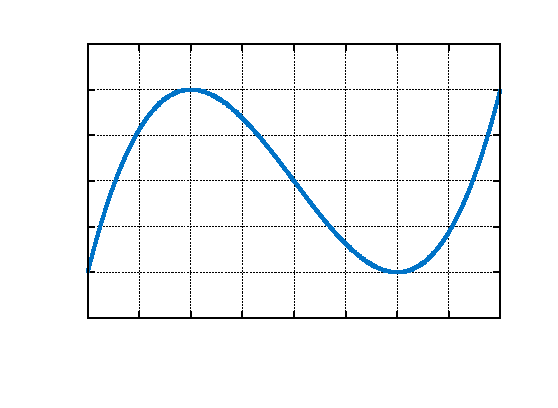
\includegraphics{calc12ex48}}%
    \gplfronttext
  \end{picture}%
\endgroup

\end{center}
\end{exmp}\vspace{-2mm}
\divider
\newpage
\begin{exmp}\label{exmp:graph2}
\noindent Sketch the graph of $f(x) ~=~ \frac{-x}{1 ~+~ x^2}$. Find all
local maxima and minima, inflection points, where the function is increasing or
decreasing, and where the function is concave up or concave down. Also indicate
any asymptotes.\vspace{1mm}
\par\noindent\emph{Solution:} Since $f'(x) = \frac{x^2 - 1}{(1+x^2)^2}$
then $x=1$ and $x=-1$ are the only critical points. And since
$f''(x) = \frac{2x\,(3 - x^2)}{(1+x^2)^3}$
then $f''(1) = \frac{1}{2} > 0$ and $f''(-1) = -\frac{1}{2} < 0$. So by the
Second Derivative Test, $f$ has a local minimum at $x=1$ and a local maximum at
$x=-1$. Since $f''(x) > 0$ for $x<-\sqrt{3}$,  $f''(x) < 0$ for $-\sqrt{3}<x<0$,
$f''(x) > 0$ for $0<x<\sqrt{3}$, and $f''(x) < 0$ for $x>\sqrt{3}$, then
$x=0,\pm\sqrt{3}$ are inflection points, $f$ is concave up for $x<-\sqrt{3}$
and for $0<x<\sqrt{3}$, and $f$ is concave down for $-\sqrt{3}<x<0$ and for
$x>\sqrt{3}$. Since $f'(x)>0$ for $x<-1$ and $x>1$ then $f$ is increasing for
$\abs{x} > 1$. And $f'(x)<0$ for $-1<x<1$ means $f$ is decreasing for
$\abs{x}<1$. Finally, since $\displaystyle\lim_{x \to \infty} f(x) = 0$ and
$\displaystyle\lim_{x \to -\infty} f(x) = 0$ then the $x$-axis ($y=0$)
is a horizontal asymptote. There are no vertical asymptotes (why?).

\par\noindent The graph is shown below:

\begin{center}
% GNUPLOT: LaTeX picture with Postscript
\begingroup
\footnotesize
  \makeatletter
  \providecommand\color[2][]{%
    \GenericError{(gnuplot) \space\space\space\@spaces}{%
      Package color not loaded in conjunction with
      terminal option `colourtext'%
    }{See the gnuplot documentation for explanation.%
    }{Either use 'blacktext' in gnuplot or load the package
      color.sty in LaTeX.}%
    \renewcommand\color[2][]{}%
  }%
  \providecommand\includegraphics[2][]{%
    \GenericError{(gnuplot) \space\space\space\@spaces}{%
      Package graphicx or graphics not loaded%
    }{See the gnuplot documentation for explanation.%
    }{The gnuplot epslatex terminal needs graphicx.sty or graphics.sty.}%
    \renewcommand\includegraphics[2][]{}%
  }%
  \providecommand\rotatebox[2]{#2}%
  \@ifundefined{ifGPcolor}{%
    \newif\ifGPcolor
    \GPcolortrue
  }{}%
  \@ifundefined{ifGPblacktext}{%
    \newif\ifGPblacktext
    \GPblacktexttrue
  }{}%
  % define a \g@addto@macro without @ in the name:
  \let\gplgaddtomacro\g@addto@macro
  % define empty templates for all commands taking text:
  \gdef\gplbacktext{}%
  \gdef\gplfronttext{}%
  \makeatother
  \ifGPblacktext
    % no textcolor at all
    \def\colorrgb#1{}%
    \def\colorgray#1{}%
  \else
    % gray or color?
    \ifGPcolor
      \def\colorrgb#1{\color[rgb]{#1}}%
      \def\colorgray#1{\color[gray]{#1}}%
      \expandafter\def\csname LTw\endcsname{\color{white}}%
      \expandafter\def\csname LTb\endcsname{\color{black}}%
      \expandafter\def\csname LTa\endcsname{\color{black}}%
      \expandafter\def\csname LT0\endcsname{\color[rgb]{1,0,0}}%
      \expandafter\def\csname LT1\endcsname{\color[rgb]{0,1,0}}%
      \expandafter\def\csname LT2\endcsname{\color[rgb]{0,0,1}}%
      \expandafter\def\csname LT3\endcsname{\color[rgb]{1,0,1}}%
      \expandafter\def\csname LT4\endcsname{\color[rgb]{0,1,1}}%
      \expandafter\def\csname LT5\endcsname{\color[rgb]{1,1,0}}%
      \expandafter\def\csname LT6\endcsname{\color[rgb]{0,0,0}}%
      \expandafter\def\csname LT7\endcsname{\color[rgb]{1,0.3,0}}%
      \expandafter\def\csname LT8\endcsname{\color[rgb]{0.5,0.5,0.5}}%
    \else
      % gray
      \def\colorrgb#1{\color{black}}%
      \def\colorgray#1{\color[gray]{#1}}%
      \expandafter\def\csname LTw\endcsname{\color{white}}%
      \expandafter\def\csname LTb\endcsname{\color{black}}%
      \expandafter\def\csname LTa\endcsname{\color{black}}%
      \expandafter\def\csname LT0\endcsname{\color{black}}%
      \expandafter\def\csname LT1\endcsname{\color{black}}%
      \expandafter\def\csname LT2\endcsname{\color{black}}%
      \expandafter\def\csname LT3\endcsname{\color{black}}%
      \expandafter\def\csname LT4\endcsname{\color{black}}%
      \expandafter\def\csname LT5\endcsname{\color{black}}%
      \expandafter\def\csname LT6\endcsname{\color{black}}%
      \expandafter\def\csname LT7\endcsname{\color{black}}%
      \expandafter\def\csname LT8\endcsname{\color{black}}%
    \fi
  \fi
    \setlength{\unitlength}{0.0500bp}%
    \ifx\gptboxheight\undefined%
      \newlength{\gptboxheight}%
      \newlength{\gptboxwidth}%
      \newsavebox{\gptboxtext}%
    \fi%
    \setlength{\fboxrule}{0.5pt}%
    \setlength{\fboxsep}{1pt}%
\begin{picture}(5040.00,3600.00)%
    \gplgaddtomacro\gplbacktext{%
      \csname LTb\endcsname%
      \put(946,704){\makebox(0,0)[r]{\strut{}$-1$}}%
      \csname LTb\endcsname%
      \put(946,1362){\makebox(0,0)[r]{\strut{}$-0.5$}}%
      \csname LTb\endcsname%
      \put(946,2020){\makebox(0,0)[r]{\strut{}$0$}}%
      \csname LTb\endcsname%
      \put(946,2677){\makebox(0,0)[r]{\strut{}$0.5$}}%
      \csname LTb\endcsname%
      \put(946,3335){\makebox(0,0)[r]{\strut{}$1$}}%
      \csname LTb\endcsname%
      \put(1078,484){\makebox(0,0){\strut{}$-4$}}%
      \csname LTb\endcsname%
      \put(1524,484){\makebox(0,0){\strut{}$-3$}}%
      \csname LTb\endcsname%
      \put(1969,484){\makebox(0,0){\strut{}$-2$}}%
      \csname LTb\endcsname%
      \put(2415,484){\makebox(0,0){\strut{}$-1$}}%
      \csname LTb\endcsname%
      \put(2861,484){\makebox(0,0){\strut{}$0$}}%
      \csname LTb\endcsname%
      \put(3306,484){\makebox(0,0){\strut{}$1$}}%
      \csname LTb\endcsname%
      \put(3752,484){\makebox(0,0){\strut{}$2$}}%
      \csname LTb\endcsname%
      \put(4197,484){\makebox(0,0){\strut{}$3$}}%
      \csname LTb\endcsname%
      \put(4643,484){\makebox(0,0){\strut{}$4$}}%
    }%
    \gplgaddtomacro\gplfronttext{%
      \csname LTb\endcsname%
      \put(176,2019){\rotatebox{-270}{\makebox(0,0){\strut{}$y$}}}%
      \put(2860,154){\makebox(0,0){\strut{}$x$}}%
    }%
    \gplbacktext
    \put(0,0){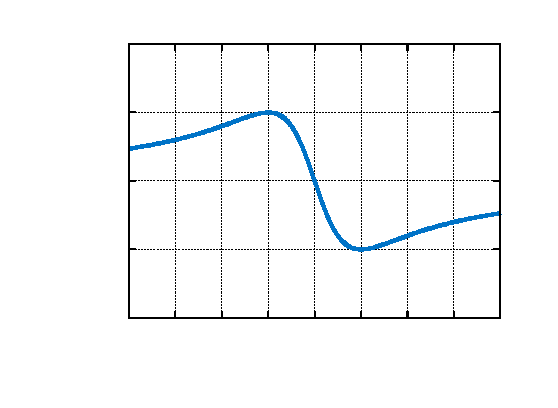
\includegraphics{calc12ex49}}%
    \gplfronttext
  \end{picture}%
\endgroup

\end{center}
\end{exmp}
\divider
\vspace{3mm}

If the Second Derivative Test fails then one alternative is the
following test:\index{First Derivative Test}

\statethm{thm:firstderivtest}{\textbf{First Derivative Test}: For a continuous
function $f$ on an interval $I$, let $x=c$ be a number in $I$ such that
$f(c)$ is defined, and either $f'(c)=0$ or $f'(c)$ does not exist. Then:
\begin{enumerate}[\bfseries (a)]
 \item If $f'(x)$ changes from negative to positive around $x=c$ then $f$ has a
  local minimum at $x=c$.
 \item If $f'(x)$ changes from positive to negative around $x=c$ then $f$ has a
  local maximum at $x=c$.
\end{enumerate}}
This test merely states the obvious: a function decreases then increases around
a minimum, and it increases then decreases around a maximum.

\begin{exmp}\label{exmp:graph3}
\parpic[r]{% GNUPLOT: LaTeX picture with Postscript
\begingroup
\footnotesize
  \makeatletter
  \providecommand\color[2][]{%
    \GenericError{(gnuplot) \space\space\space\@spaces}{%
      Package color not loaded in conjunction with
      terminal option `colourtext'%
    }{See the gnuplot documentation for explanation.%
    }{Either use 'blacktext' in gnuplot or load the package
      color.sty in LaTeX.}%
    \renewcommand\color[2][]{}%
  }%
  \providecommand\includegraphics[2][]{%
    \GenericError{(gnuplot) \space\space\space\@spaces}{%
      Package graphicx or graphics not loaded%
    }{See the gnuplot documentation for explanation.%
    }{The gnuplot epslatex terminal needs graphicx.sty or graphics.sty.}%
    \renewcommand\includegraphics[2][]{}%
  }%
  \providecommand\rotatebox[2]{#2}%
  \@ifundefined{ifGPcolor}{%
    \newif\ifGPcolor
    \GPcolortrue
  }{}%
  \@ifundefined{ifGPblacktext}{%
    \newif\ifGPblacktext
    \GPblacktexttrue
  }{}%
  % define a \g@addto@macro without @ in the name:
  \let\gplgaddtomacro\g@addto@macro
  % define empty templates for all commands taking text:
  \gdef\gplbacktext{}%
  \gdef\gplfronttext{}%
  \makeatother
  \ifGPblacktext
    % no textcolor at all
    \def\colorrgb#1{}%
    \def\colorgray#1{}%
  \else
    % gray or color?
    \ifGPcolor
      \def\colorrgb#1{\color[rgb]{#1}}%
      \def\colorgray#1{\color[gray]{#1}}%
      \expandafter\def\csname LTw\endcsname{\color{white}}%
      \expandafter\def\csname LTb\endcsname{\color{black}}%
      \expandafter\def\csname LTa\endcsname{\color{black}}%
      \expandafter\def\csname LT0\endcsname{\color[rgb]{1,0,0}}%
      \expandafter\def\csname LT1\endcsname{\color[rgb]{0,1,0}}%
      \expandafter\def\csname LT2\endcsname{\color[rgb]{0,0,1}}%
      \expandafter\def\csname LT3\endcsname{\color[rgb]{1,0,1}}%
      \expandafter\def\csname LT4\endcsname{\color[rgb]{0,1,1}}%
      \expandafter\def\csname LT5\endcsname{\color[rgb]{1,1,0}}%
      \expandafter\def\csname LT6\endcsname{\color[rgb]{0,0,0}}%
      \expandafter\def\csname LT7\endcsname{\color[rgb]{1,0.3,0}}%
      \expandafter\def\csname LT8\endcsname{\color[rgb]{0.5,0.5,0.5}}%
    \else
      % gray
      \def\colorrgb#1{\color{black}}%
      \def\colorgray#1{\color[gray]{#1}}%
      \expandafter\def\csname LTw\endcsname{\color{white}}%
      \expandafter\def\csname LTb\endcsname{\color{black}}%
      \expandafter\def\csname LTa\endcsname{\color{black}}%
      \expandafter\def\csname LT0\endcsname{\color{black}}%
      \expandafter\def\csname LT1\endcsname{\color{black}}%
      \expandafter\def\csname LT2\endcsname{\color{black}}%
      \expandafter\def\csname LT3\endcsname{\color{black}}%
      \expandafter\def\csname LT4\endcsname{\color{black}}%
      \expandafter\def\csname LT5\endcsname{\color{black}}%
      \expandafter\def\csname LT6\endcsname{\color{black}}%
      \expandafter\def\csname LT7\endcsname{\color{black}}%
      \expandafter\def\csname LT8\endcsname{\color{black}}%
    \fi
  \fi
    \setlength{\unitlength}{0.0500bp}%
    \ifx\gptboxheight\undefined%
      \newlength{\gptboxheight}%
      \newlength{\gptboxwidth}%
      \newsavebox{\gptboxtext}%
    \fi%
    \setlength{\fboxrule}{0.5pt}%
    \setlength{\fboxsep}{1pt}%
\begin{picture}(3600.00,2160.00)%
    \gplgaddtomacro\gplbacktext{%
      \csname LTb\endcsname%
      \put(814,704){\makebox(0,0)[r]{\strut{}$0$}}%
      \csname LTb\endcsname%
      \put(814,874){\makebox(0,0)[r]{\strut{}$0.2$}}%
      \csname LTb\endcsname%
      \put(814,1044){\makebox(0,0)[r]{\strut{}$0.4$}}%
      \csname LTb\endcsname%
      \put(814,1214){\makebox(0,0)[r]{\strut{}$0.6$}}%
      \csname LTb\endcsname%
      \put(814,1385){\makebox(0,0)[r]{\strut{}$0.8$}}%
      \csname LTb\endcsname%
      \put(814,1555){\makebox(0,0)[r]{\strut{}$1$}}%
      \csname LTb\endcsname%
      \put(814,1725){\makebox(0,0)[r]{\strut{}$1.2$}}%
      \csname LTb\endcsname%
      \put(814,1895){\makebox(0,0)[r]{\strut{}$1.4$}}%
      \csname LTb\endcsname%
      \put(946,484){\makebox(0,0){\strut{}$-2$}}%
      \csname LTb\endcsname%
      \put(1228,484){\makebox(0,0){\strut{}$-1.5$}}%
      \csname LTb\endcsname%
      \put(1510,484){\makebox(0,0){\strut{}$-1$}}%
      \csname LTb\endcsname%
      \put(1792,484){\makebox(0,0){\strut{}$-0.5$}}%
      \csname LTb\endcsname%
      \put(2075,484){\makebox(0,0){\strut{}$0$}}%
      \csname LTb\endcsname%
      \put(2357,484){\makebox(0,0){\strut{}$0.5$}}%
      \csname LTb\endcsname%
      \put(2639,484){\makebox(0,0){\strut{}$1$}}%
      \csname LTb\endcsname%
      \put(2921,484){\makebox(0,0){\strut{}$1.5$}}%
      \csname LTb\endcsname%
      \put(3203,484){\makebox(0,0){\strut{}$2$}}%
    }%
    \gplgaddtomacro\gplfronttext{%
      \csname LTb\endcsname%
      \put(176,1299){\rotatebox{-270}{\makebox(0,0){\strut{}$y$}}}%
      \put(2074,154){\makebox(0,0){\strut{}$x$}}%
    }%
    \gplbacktext
    \put(0,0){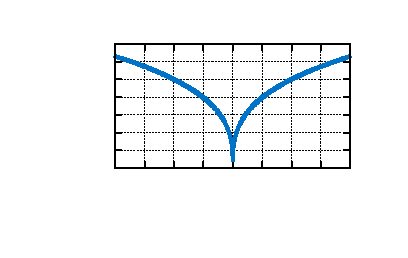
\includegraphics{calc12ex410}}%
    \gplfronttext
  \end{picture}%
\endgroup
}
\noindent Sketch the graph of $f(x) = x^{2/3}$.\vspace{1mm}
\par\noindent\emph{Solution:} Clearly $f(x)$ is continuous for all $x$,
including $x=0$ (since $f(0)=0$), but $f'(x) = \frac{2}{3\,\sqrt[3]{x}}$ is not
defined at $x=0$. Since $f'(x)$ changes from negative to positive around $x=0$
($f'(x) < 0$ when $x < 0$ and $f'(x) > 0$ when $x > 0$), then by the First
Derivative Test $f$ has a local minimum at $x=0$. Since $f''(x) = -\,
\frac{2}{9\,x^{4/3}} < 0$ for all $x \ne 0$, then $f$ is always concave down.
There are no vertical or horizontal asymptotes. The graph is shown on the
right.\vspace{2mm}
\picskip{0}
\par\noindent Note that the Second Derivative Test could not be used for this
function, since $f'(x) \ne 0$ for all $x$ (notice also that $f''(x)$ is not
defined at $x=0$).
\end{exmp}
\divider
\vspace{3mm}

A more complete alternative to the Second Derivative Test is the
following:\footnote{For a proof, see pp.10-11 in
\textsc{Koo, D.}, \emph{Elements of Optimization}, New York: Springer-Verlag,
1977.}\index{Nth Derivative Test@N\textsuperscript{th} Derivative Test}

\statethm{thm:nderivtest}{\textbf{N\textsuperscript{th} Derivative Test}: A
non-constant
function $f$ with continuous derivatives of all orders up to and including
$n >1$ at $x=c$ has either a local minimum, local maximum or inflection point at
$x=c$ if and only if
\[
f^{(k)}(c) ~=~ 0 ~~\text{for $k=1$, $2$, $\ldots$, $n-1$}
\quad\text{and}\quad f^{(n)}(c) ~\ne~ 0
\]
(i.e. the $n^{\text{th}}$ derivative is the first nonzero derivative at $x=c$).
If so, then:

\begin{enumerate}[\bfseries (a)]
 \item If $n>1$ is even and $f^{(n)}(c) > 0$ then $f$ has a
  local minimum at $x=c$.
 \item If $n>1$ is even and $f^{(n)}(c) < 0$ then $f$ has a
  local maximum at $x=c$.
 \item If $n>1$ is odd then $f$ has an inflection point at $x=c$.
\end{enumerate}}
Note that the Second Derivative Test is the special case where $n=2$ in the
N\textsuperscript{th} Derivative Test. Though this test gives necessary
and sufficient conditions for a local maximum, local minimum, and inflection
point, calculating the first $n$ derivatives can be complicated if $n$ is large
and the given function is not simple.

\begin{exmp}\label{exmp:graph4}
The Second Derivative Test fails for $f(x)=x^4$ at the critical point $x=0$,
since $f''(0)=0$. But the first 4 derivatives of $f(x)=x^4$ are $f'(x)=4x^3$,
$f''(x)=12x^2$, $f^{(3)}(x)=24x$, and $f^{(4)}(x)=24$, which are all continuous
and
\[
f^{(k)}(0) ~=~ 0 ~~\text{for $k=1$, $2$, $3$}
\quad\text{and}\quad f^{(4)}(0) ~=~ 24 ~\ne~ 0 ~.
\]
So by the
N\textsuperscript{th} Derivative Test, since $n=4$ is even and $f^{(4)}(0)=24>0$
then $f(x)=x^4$ has a local minimum at $x=0$. Note that $f(x) \ge 0 = f(0)$ for
all $x$, so $x = 0$ is actually a global minimum for $f$.
\end{exmp}
\divider
\newpage
A common practice in many fields of science and engineering is to combine
multiple named constants (e.g. $\pi$) or variables in a function into one
variable and then sketch a graph of that function. The example below illustrates
the technique.

\begin{exmp}\label{exmp:graph5}
\noindent A hydrogen atom has one electron, and the probability of finding the
electron in the ground state of the hydrogen atom between radii $r$ and $r+\dr$
is $D(r)\,\dr$, where $\dr$ is an infinitesimal change in the radius $r$ (the
distance from the electron to the nucleus), $D(r)$ is the \emph{radial
probability density function}
\[
D(r) ~=~ \frac{4}{a_0^3}\,r^2 e^{-2r/a_0}
\]
and $a_0 \approx 5.291772 \times 10^{-11}$ m is the \emph{Bohr radius}\index{Bohr
radius}. It is useful to analyze this function in terms of $r \ge 0$
in relation to the Bohr radius $a_0$ (e.g.
$r= 0.5a_0$, $a_0$, $2a_0$, $3a_0$). To do this, let $x = \frac{r}{a_0}$, so that
\[
D(r) ~=~ \frac{4}{a_0}\,\left(\frac{r}{a_0}\right)^2 e^{-2\left(\frac{r}{a_0}\right)}
\quad\Rightarrow\quad
a_0\,D(x) ~=~ 4x^2 e^{-2x}
\]
and then sketch the graph of $a_0\,D(x)$, which is shown below:

\begin{center}
% GNUPLOT: LaTeX picture with Postscript
\begingroup
\footnotesize
  \makeatletter
  \providecommand\color[2][]{%
    \GenericError{(gnuplot) \space\space\space\@spaces}{%
      Package color not loaded in conjunction with
      terminal option `colourtext'%
    }{See the gnuplot documentation for explanation.%
    }{Either use 'blacktext' in gnuplot or load the package
      color.sty in LaTeX.}%
    \renewcommand\color[2][]{}%
  }%
  \providecommand\includegraphics[2][]{%
    \GenericError{(gnuplot) \space\space\space\@spaces}{%
      Package graphicx or graphics not loaded%
    }{See the gnuplot documentation for explanation.%
    }{The gnuplot epslatex terminal needs graphicx.sty or graphics.sty.}%
    \renewcommand\includegraphics[2][]{}%
  }%
  \providecommand\rotatebox[2]{#2}%
  \@ifundefined{ifGPcolor}{%
    \newif\ifGPcolor
    \GPcolortrue
  }{}%
  \@ifundefined{ifGPblacktext}{%
    \newif\ifGPblacktext
    \GPblacktexttrue
  }{}%
  % define a \g@addto@macro without @ in the name:
  \let\gplgaddtomacro\g@addto@macro
  % define empty templates for all commands taking text:
  \gdef\gplbacktext{}%
  \gdef\gplfronttext{}%
  \makeatother
  \ifGPblacktext
    % no textcolor at all
    \def\colorrgb#1{}%
    \def\colorgray#1{}%
  \else
    % gray or color?
    \ifGPcolor
      \def\colorrgb#1{\color[rgb]{#1}}%
      \def\colorgray#1{\color[gray]{#1}}%
      \expandafter\def\csname LTw\endcsname{\color{white}}%
      \expandafter\def\csname LTb\endcsname{\color{black}}%
      \expandafter\def\csname LTa\endcsname{\color{black}}%
      \expandafter\def\csname LT0\endcsname{\color[rgb]{1,0,0}}%
      \expandafter\def\csname LT1\endcsname{\color[rgb]{0,1,0}}%
      \expandafter\def\csname LT2\endcsname{\color[rgb]{0,0,1}}%
      \expandafter\def\csname LT3\endcsname{\color[rgb]{1,0,1}}%
      \expandafter\def\csname LT4\endcsname{\color[rgb]{0,1,1}}%
      \expandafter\def\csname LT5\endcsname{\color[rgb]{1,1,0}}%
      \expandafter\def\csname LT6\endcsname{\color[rgb]{0,0,0}}%
      \expandafter\def\csname LT7\endcsname{\color[rgb]{1,0.3,0}}%
      \expandafter\def\csname LT8\endcsname{\color[rgb]{0.5,0.5,0.5}}%
    \else
      % gray
      \def\colorrgb#1{\color{black}}%
      \def\colorgray#1{\color[gray]{#1}}%
      \expandafter\def\csname LTw\endcsname{\color{white}}%
      \expandafter\def\csname LTb\endcsname{\color{black}}%
      \expandafter\def\csname LTa\endcsname{\color{black}}%
      \expandafter\def\csname LT0\endcsname{\color{black}}%
      \expandafter\def\csname LT1\endcsname{\color{black}}%
      \expandafter\def\csname LT2\endcsname{\color{black}}%
      \expandafter\def\csname LT3\endcsname{\color{black}}%
      \expandafter\def\csname LT4\endcsname{\color{black}}%
      \expandafter\def\csname LT5\endcsname{\color{black}}%
      \expandafter\def\csname LT6\endcsname{\color{black}}%
      \expandafter\def\csname LT7\endcsname{\color{black}}%
      \expandafter\def\csname LT8\endcsname{\color{black}}%
    \fi
  \fi
    \setlength{\unitlength}{0.0500bp}%
    \ifx\gptboxheight\undefined%
      \newlength{\gptboxheight}%
      \newlength{\gptboxwidth}%
      \newsavebox{\gptboxtext}%
    \fi%
    \setlength{\fboxrule}{0.5pt}%
    \setlength{\fboxsep}{1pt}%
\begin{picture}(5040.00,3600.00)%
    \gplgaddtomacro\gplbacktext{%
      \csname LTb\endcsname%
      \put(814,704){\makebox(0,0)[r]{\strut{}$0$}}%
      \csname LTb\endcsname%
      \put(814,1143){\makebox(0,0)[r]{\strut{}$0.1$}}%
      \csname LTb\endcsname%
      \put(814,1581){\makebox(0,0)[r]{\strut{}$0.2$}}%
      \csname LTb\endcsname%
      \put(814,2020){\makebox(0,0)[r]{\strut{}$0.3$}}%
      \csname LTb\endcsname%
      \put(814,2458){\makebox(0,0)[r]{\strut{}$0.4$}}%
      \csname LTb\endcsname%
      \put(814,2896){\makebox(0,0)[r]{\strut{}$0.5$}}%
      \csname LTb\endcsname%
      \put(814,3335){\makebox(0,0)[r]{\strut{}$0.6$}}%
      \csname LTb\endcsname%
      \put(946,484){\makebox(0,0){\strut{}$0$}}%
      \csname LTb\endcsname%
      \put(1562,484){\makebox(0,0){\strut{}$1$}}%
      \csname LTb\endcsname%
      \put(2178,484){\makebox(0,0){\strut{}$2$}}%
      \csname LTb\endcsname%
      \put(2795,484){\makebox(0,0){\strut{}$3$}}%
      \csname LTb\endcsname%
      \put(3411,484){\makebox(0,0){\strut{}$4$}}%
      \csname LTb\endcsname%
      \put(4027,484){\makebox(0,0){\strut{}$5$}}%
      \csname LTb\endcsname%
      \put(4643,484){\makebox(0,0){\strut{}$6$}}%
    }%
    \gplgaddtomacro\gplfronttext{%
      \csname LTb\endcsname%
      \put(176,2019){\rotatebox{-270}{\makebox(0,0){\strut{}$a_0 D\left(\tfrac{r}{a_0}\right)$}}}%
      \put(2794,154){\makebox(0,0){\strut{}$\frac{r}{a_0}$}}%
    }%
    \gplbacktext
    \put(0,0){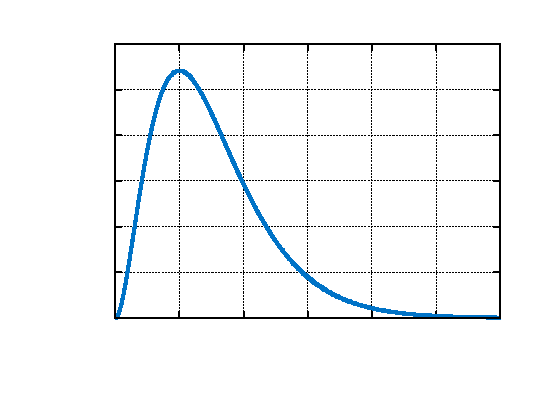
\includegraphics{calc12ex412}}%
    \gplfronttext
  \end{picture}%
\endgroup

\end{center}

\noindent From the graph it looks like $x=1$ (i.e. $r = a_0$) is a local (and
global) maximum, so that the electron is most likely to be found near
$r = a_0$, and the probability drops off dramatically past a distance
$r = 3a_0$. In the exercises you will be asked to show that $r = a_0$ is indeed
a local maximum and that the inflection points are
$r = \left(1 \pm \frac{1}{\sqrt{2}}\right)\,a_0$.\vspace{2mm}

\par\noindent Note that the right side of the formula
$a_0\,D(x) = 4x^2 e^{-2x}$ does not involve $a_0$, which was multiplied
over to the left side. In general that is the strategy when dealing with
these sorts of functions where variables and constants are combined. In this
case the stray constant $a_0$ can be multiplied with $D$ since that will not
affect the location of critical and inflection points, nor fundamentally alter
the general shape of the graph.
\end{exmp}
\divider
\newpage
\begin{exmp}\label{exmp:thermalex}
\noindent For a single particle with two states---energy 0 and energy
$\epsilon$---in thermal contact with a reservoir at temperature $\tau$, the
average energy $U$ and heat capacity $C_V$ are given by
\[
U ~=~ \epsilon\,\frac{e^{-\epsilon/\tau}}{1 + e^{-\epsilon/\tau}} \quad\text{and}\quad
C_V ~=~ k_B\,\left(\frac{\epsilon}{\tau}\right)^2 \frac{e^{\epsilon/\tau}}{\left(1 + e^{\epsilon/\tau}\right)^2}
\]
where $k_B \approx 1.38065 \times 10^{\text{$-$}23}$ J/K is the
\emph{Boltzmann constant}. The graph below shows both quantities as functions
of $\tau/\epsilon$ (\emph{not} $\epsilon/\tau$, as you might
expect). See Exercise \ref{exer:thermalex}.\vspace{-3mm}

\begin{center}
% GNUPLOT: LaTeX picture with Postscript
\begingroup
  \makeatletter
  \providecommand\color[2][]{%
    \GenericError{(gnuplot) \space\space\space\@spaces}{%
      Package color not loaded in conjunction with
      terminal option `colourtext'%
    }{See the gnuplot documentation for explanation.%
    }{Either use 'blacktext' in gnuplot or load the package
      color.sty in LaTeX.}%
    \renewcommand\color[2][]{}%
  }%
  \providecommand\includegraphics[2][]{%
    \GenericError{(gnuplot) \space\space\space\@spaces}{%
      Package graphicx or graphics not loaded%
    }{See the gnuplot documentation for explanation.%
    }{The gnuplot epslatex terminal needs graphicx.sty or graphics.sty.}%
    \renewcommand\includegraphics[2][]{}%
  }%
  \providecommand\rotatebox[2]{#2}%
  \@ifundefined{ifGPcolor}{%
    \newif\ifGPcolor
    \GPcolortrue
  }{}%
  \@ifundefined{ifGPblacktext}{%
    \newif\ifGPblacktext
    \GPblacktexttrue
  }{}%
  % define a \g@addto@macro without @ in the name:
  \let\gplgaddtomacro\g@addto@macro
  % define empty templates for all commands taking text:
  \gdef\gplbacktext{}%
  \gdef\gplfronttext{}%
  \makeatother
  \ifGPblacktext
    % no textcolor at all
    \def\colorrgb#1{}%
    \def\colorgray#1{}%
  \else
    % gray or color?
    \ifGPcolor
      \def\colorrgb#1{\color[rgb]{#1}}%
      \def\colorgray#1{\color[gray]{#1}}%
      \expandafter\def\csname LTw\endcsname{\color{white}}%
      \expandafter\def\csname LTb\endcsname{\color{black}}%
      \expandafter\def\csname LTa\endcsname{\color{black}}%
      \expandafter\def\csname LT0\endcsname{\color[rgb]{1,0,0}}%
      \expandafter\def\csname LT1\endcsname{\color[rgb]{0,1,0}}%
      \expandafter\def\csname LT2\endcsname{\color[rgb]{0,0,1}}%
      \expandafter\def\csname LT3\endcsname{\color[rgb]{1,0,1}}%
      \expandafter\def\csname LT4\endcsname{\color[rgb]{0,1,1}}%
      \expandafter\def\csname LT5\endcsname{\color[rgb]{1,1,0}}%
      \expandafter\def\csname LT6\endcsname{\color[rgb]{0,0,0}}%
      \expandafter\def\csname LT7\endcsname{\color[rgb]{1,0.3,0}}%
      \expandafter\def\csname LT8\endcsname{\color[rgb]{0.5,0.5,0.5}}%
    \else
      % gray
      \def\colorrgb#1{\color{black}}%
      \def\colorgray#1{\color[gray]{#1}}%
      \expandafter\def\csname LTw\endcsname{\color{white}}%
      \expandafter\def\csname LTb\endcsname{\color{black}}%
      \expandafter\def\csname LTa\endcsname{\color{black}}%
      \expandafter\def\csname LT0\endcsname{\color{black}}%
      \expandafter\def\csname LT1\endcsname{\color{black}}%
      \expandafter\def\csname LT2\endcsname{\color{black}}%
      \expandafter\def\csname LT3\endcsname{\color{black}}%
      \expandafter\def\csname LT4\endcsname{\color{black}}%
      \expandafter\def\csname LT5\endcsname{\color{black}}%
      \expandafter\def\csname LT6\endcsname{\color{black}}%
      \expandafter\def\csname LT7\endcsname{\color{black}}%
      \expandafter\def\csname LT8\endcsname{\color{black}}%
    \fi
  \fi
    \setlength{\unitlength}{0.0500bp}%
    \ifx\gptboxheight\undefined%
      \newlength{\gptboxheight}%
      \newlength{\gptboxwidth}%
      \newsavebox{\gptboxtext}%
    \fi%
    \setlength{\fboxrule}{0.5pt}%
    \setlength{\fboxsep}{1pt}%
\begin{picture}(7200.00,4032.00)%
    \gplgaddtomacro\gplbacktext{%
      \csname LTb\endcsname%
      \put(726,704){\makebox(0,0)[r]{\strut{}$0$}}%
      \put(726,971){\makebox(0,0)[r]{\strut{}$0.05$}}%
      \put(726,1237){\makebox(0,0)[r]{\strut{}$0.1$}}%
      \put(726,1504){\makebox(0,0)[r]{\strut{}$0.15$}}%
      \put(726,1771){\makebox(0,0)[r]{\strut{}$0.2$}}%
      \put(726,2038){\makebox(0,0)[r]{\strut{}$0.25$}}%
      \put(726,2304){\makebox(0,0)[r]{\strut{}$0.3$}}%
      \put(726,2571){\makebox(0,0)[r]{\strut{}$0.35$}}%
      \put(726,2838){\makebox(0,0)[r]{\strut{}$0.4$}}%
      \put(726,3104){\makebox(0,0)[r]{\strut{}$0.45$}}%
      \put(726,3371){\makebox(0,0)[r]{\strut{}$0.5$}}%
      \put(858,484){\makebox(0,0){\strut{}$0$}}%
      \put(2047,484){\makebox(0,0){\strut{}$1$}}%
      \put(3236,484){\makebox(0,0){\strut{}$2$}}%
      \put(4425,484){\makebox(0,0){\strut{}$3$}}%
      \put(5614,484){\makebox(0,0){\strut{}$4$}}%
      \put(6803,484){\makebox(0,0){\strut{}$5$}}%
    }%
    \gplgaddtomacro\gplfronttext{%
      \csname LTb\endcsname%
      \put(3830,154){\makebox(0,0){\strut{}$\tau/\epsilon$}}%
      \put(3830,3701){\makebox(0,0){\strut{}Average Energy $U/\epsilon$ vs Heat Capacity $C_V/k_B$}}%
      \csname LTb\endcsname%
      \put(5816,2509){\makebox(0,0)[r]{\strut{}$U/\epsilon = \dfrac{e^{-\epsilon/\tau}}{1 + e^{-\epsilon/\tau}}$}}%
      \csname LTb\endcsname%
      \put(5816,1564){\makebox(0,0)[r]{\strut{}$C_V/k_B = \left(\dfrac{\epsilon}{\tau}\right)^2 \dfrac{e^{\epsilon/\tau}}{\left(1 + e^{\epsilon/\tau}\right)^2}$}}%
    }%
    \gplbacktext
    \put(0,0){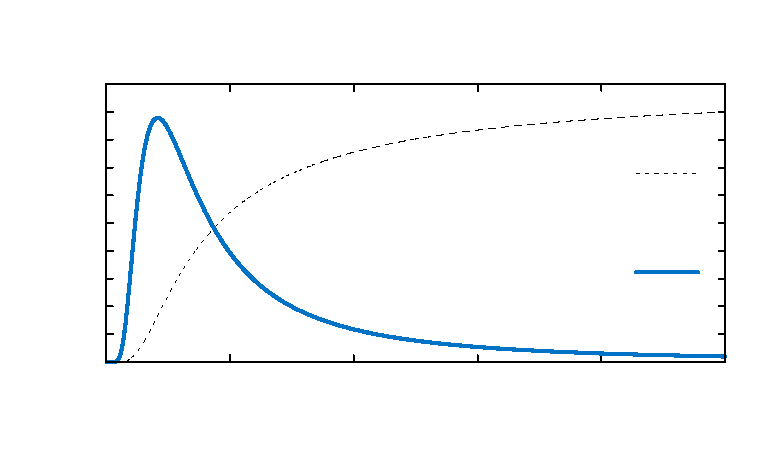
\includegraphics{thermalex}}%
    \gplfronttext
  \end{picture}%
\endgroup

\end{center}
\end{exmp}\vspace{-4mm}
\divider
\vspace{3mm}
\startexercises\label{sec4dot2}
{\small
\probs{A}
\par\noindent For Exercises 1-8 sketch the graph of the given function. Find all
local maxima and minima, inflection points, where the function is increasing or
decreasing, where the function is concave up or concave down, and indicate any
asymptotes.
\begin{enumerate}[\bfseries 1.]
 \begin{multicols}{4}
  \item $f(x) ~=~ x^3 - 3x\vphantom{;e^{-x^2}}$
  \item $f(x) ~=~ x^3 - 3x^2 + 1\vphantom{;e^{-x^2}}$
  \item $f(x) ~=~ xe^{-x}\vphantom{;e^{-x^2}}$
  \item $f(x) ~=~ x^2 \;e^{-x^2}$
 \end{multicols}
 \begin{multicols}{4}
  \item $f(x) ~=~ \dfrac{1}{1 ~+~ x^2}\vphantom{\dfrac{e^{-x} ~-~ e^{-2x}}{2}}$
  \item $f(x) ~=~ \dfrac{x^2}{(x - 1)^2}\vphantom{\dfrac{e^{-x} ~-~ e^{-2x}}{2}}$
  \item $f(x) ~=~ \dfrac{e^{-x} ~-~ e^{-2x}}{2}$
  \item $f(x) ~=~ e^{-x}\;\sin\,x\vphantom{\dfrac{e^{-x} ~-~ e^{-2x}}{2}}$
 \end{multicols}
  \item\label{exer:thermalex} Write $U/\epsilon$ and $C_V/k_B$ from Example
   \ref{exmp:thermalex} as functions of $x=\tau/\epsilon$. You do not need to
   sketch the graphs.
 \item Show that the function $D(r) = \frac{4}{a_0^3}\,r^2 e^{-2r/a_0}$ from Example
  \ref{exmp:graph5} has a local maximum at $r=a_0$ and inflection points at
  $r = \left(1 \pm \frac{1}{\sqrt{2}}\right)\,a_0$.
 \item Sketch the graph of \emph{Kratzer's molecular potential}
  $V(r) = -2D\,\left(\frac{a}{r} - \frac{1}{2} \frac{a^2}{r^2}\right)$ as a
  function of $x=\frac{r}{a}$, with $a > 0$ and $D > 0$ as constants.
 \item Sketch the graph of
  $f(K) = \frac{2N\sqrt{K}\,e^{-\frac{K}{kT}}}{\sqrt{\pi}\,(kT)^{3/2}}$ as a
  function of $x=\frac{K}{kT}$, with $N$, $k$ and $T$ as positive constants.
 \item Prove part (b) of the Concavity Theorem.
\end{enumerate}
}
\newpage
%Begin Section 4.3
\section{Numerical Approximation of Roots of Functions}
When finding critical points of a function $f$, you encounter the problem of
solving the equation $f'(x)=0$. The examples and exercises so far were set up
carefully so that solutions to that equation could be found in a simple closed
form. But in practice this will not always be the case---in fact it is
\emph{almost never} the case.\index{root of function}\index{function!root}
For example, finding the critical points of the function
$f(x) = \sin\,x \;-\; \frac{x^2}{2}$
entails solving the equation $f'(x) = \cos\,x \;-\; x ~=~ 0$, for which there is
no solution in a closed-form expression.

What should you do in such a situation?\footnote{Note: To ``just give up''---as
suggested semi-seriously by some students I have had---is not an option.}  One
possibility is to use the bisection method\index{bisection method} mentioned in
Section 3.3. In fact, in Example \ref{exmp:ivt} the solution to the equation
$\cos\,x = x$ (i.e. $\cos\,x \;-\; x \;=\;0$) was shown to exist in the interval
$\ival{0}{1}$, and then a demonstration of the bisection method was given to
find that solution.

The bisection method is one of many \emph{numerical methods} for finding roots
of a function (i.e. where the function is zero). Finding the critical points of
a function means finding the roots of its derivative. Though the bisection
method could be used for that purpose, convergence to each root is usually
slow.\index{Newton's method} A far more efficient method is
\textbf{Newton's method}\footnote{Sometimes called the \emph{Newton-Raphson
method}.}, whose geometric interpretation is shown in Figure \ref{fig:newton}
below.

\begin{figure}[ht]
 \centering
 \begin{tikzpicture}[>=latex,every node/.style={font=\small}]
  \draw [black!60,line width=1pt,->] (0,-1) -- (0,4.5) node[above] {$y$};
  \draw [name path=xaxis,black!60,line width=1pt,->] (-1.5,0) -- (9.5,0) node[right] {$x$};
  \draw[name path=x0vert,white] (7.5,0.4) -- (7.5,4.5);
  \draw[name path=x1vert,white] (5,0.2) -- (5,2);
  \draw[name path=curve,linecolor,line width=1.5pt] (0.5,-1) parabola (8,4.5);
  \fill [name intersections={of=curve and xaxis,by={x}}] (x) circle (2.5pt);
  \fill [name intersections={of=curve and x0vert,by={f0}}] (f0) circle (2.5pt);
  \fill [name intersections={of=curve and x1vert,by={f1}}] (f1) circle (2.5pt);
  \node[below left] at (0,0) {$0$};
  \node[above] at (6,3) {$y=f(x)$};
  \node[below] at (x) {$\bar{x}$};
  \node[below] at (7.5,0) {$x_0$};
  \draw[dashed] (7.5,0.02) -- (f0);
  \node[right] at (f0) {$(x_0,f(x_0))$};
  \draw[red,line width=0.6pt] (f0) -- (5,0.02);
  \node[below] at (5,0) {$x_1$};
  \draw[dashed] (5,0.02) -- (f1);
  \node[left] at (f1) {$(x_1,f(x_1))$};
  \draw[red,line width=0.6pt] (f1) -- (4.05,0.02);
  \node[below] at (4.05,0) {$x_2$};
 \end{tikzpicture}
 \caption[]{\quad Newton's method for finding a root $\bar{x}$ of $f(x)$}
 \label{fig:newton}
\end{figure}

\noindent The idea behind Newton's method is simple: to find a root $\bar{x}$ of
a function $f$, choose an \emph{initial guess} $x_0$ and then go up---or
down---to the curve $y=f(x)$ and draw the tangent line to the curve at the
point $(x_0,f(x_0))$. Let $x_1$ be where that tangent line intersects the
$x$-axis, as shown above; repeat this procedure on $x_1$ to get the next number
$x_2$, repeat on $x_2$ to get $x_3$, and so on. The resulting sequence of
numbers $x_0$, $x_1$, $x_2$, $x_3$, $\ldots$, will approach the root $\bar{x}$.
Convergence under certain conditions can be proved.\footnote{See pp.58-62 in
\textsc{Saaty, T.L. and J. Bram}, \emph{Nonlinear Mathematics}, New York:
McGraw-Hill, Inc., 1964.}
\newpage
The general formula for the number $x_n$ obtained after $n \ge 1$ iterations in
Newton's method can be determined by considering the formula for $x_1$. First,
the tangent line to $y=f(x)$ at the point $(x_0,f(x_0))$ has slope $f'(x_0)$, so
the equation of the line is
\begin{equation}\label{eqn:newton}
y ~-~ f(x_0) ~=~ f'(x_0)\,(x ~-~ x_0) ~.
\end{equation}
 The point $(x_1,0)$ is (by design) also on that line, so that
\[
0 ~-~ f(x_0) ~=~ f'(x_0)\,(x_1 ~-~ x_0) \quad\Rightarrow\quad
x_1 ~=~ x_0 ~-~ \frac{f(x_0)}{f'(x_0)}
\]
provided that $f'(x_0) \ne 0$. The general formula for $x_n$ is given by the
following algorithm:

\statedefn{defn:newton}{\textbf{Newton's method}: For an initial guess $x_0$,
the numbers $x_n$ for $n \ge 1$ are computed iteratively as:
\[
x_n ~=~ x_{n-1} ~-~ \frac{f(x_{n-1})}{f'(x_{n-1})} \qquad\text{for $n =1$, $2$,
$3$, $\ldots$}
\]
That is, each ``next'' number $x_n$ depends on the previous number $x_{n-1}$.
The algorithm terminates whenever $f'(x_n)=0$, or when the desired accuracy is
reached. If $f'(x_n)=0$ for some $n \ge 0$, then you could start over with a
different initial guess $x_0$.}

To implement this algorithm in a programming language (for which Newton's
method is well-suited), the following language-independent \emph{pseudocode}
can be used as a guide:

\statecor{cor:newtonalg}{\begin{center}
 \textbf{Algorithm pseudocode for Newton's method}
\end{center}
\begin{codebox}
\Procname{$\proc{Newton's method}$}
\li $N \gets \const{Number-of-iterations}$\>\>\>\>\>\>\>\>\>\Comment User supplies this value
\li $x \gets \const{initial-guess}$\>\>\>\>\>\>\>\>\>\Comment User supplies this value
\li \For $n \gets 1$ \To $N$
\li    \Do
\li       \If $f'(x) \neq 0$
\li          \Then
\li             $x \gets x ~-~ \dfrac{f(x)}{f'(x)}$
\li             print $x$
\li       \Else
\li          \Error ``division by zero''
          \End
       \End
\end{codebox}}
\newpage
\begin{exmp}\label{exmp:newt1}
\noindent Use Newton's method to find the root of $f(x) = \cos\,x - x$.\vspace{1mm}
\par\noindent\emph{Solution:} Since the root is already known to be in the
interval $\ival{0}{1}$, choose $x_0 = 1$ as the initial guess. The numbers
$x_n$ for $n \ge 1$ can be computed with a hand-held scientific calculator, but
the process is tedious and error-prone. Using a computer is far more efficient
and allows more flexibility.

For example, the algorithm is easily implemented in the Java programming
language. Save this code in a plain text file as \texttt{newton.java}:
\lstset{language=Java,showstringspaces=false,lineskip=0.3pt,xleftmargin=0.06\textwidth,
basicstyle={\small\fontfamily{fvm}\fontseries{m}\selectfont},
keywordstyle={\small\fontfamily{fvm}\fontseries{b}\selectfont},
numberstyle={\color{linenumcolor}\footnotesize\fontfamily{fvm}\fontseries{m}\selectfont},
breaklines=true,columns=fullflexible,backgroundcolor=\color{codecolor},numbers=left,
linewidth=0.95\textwidth,keepspaces=true,float=h,
caption={\quad Newton's method in Java (\texttt{newton.java})},numbersep=15pt,
label=newt1java}
\begin{lstlisting}[frame=single,framerule=0pt]
public class newton {
   public static void main(String[] args) {
      int N = Integer.parseInt(args[0]); //Number of iterations
      double x = 1.0; //initial guess
      System.out.println("n=0: " + x);
      for (int i = 1; i <= N; i++) {
         x =  x - f(x)/derivf(x);
         System.out.println("n=" + i + ": " + x);
      }
   }
 
   //Define the function f(x)
   public static double f(double x) {
      return Math.cos(x) - x;
   }

   //Define the derivative f'(x)
   public static double derivf(double x) {
      return -Math.sin(x) - 1.0;
   }
}
\end{lstlisting}
\noindent Though knowledge of Java would help, it should not be that difficult
to figure out what the above code is doing. The number of iterations $N$ is
passed as a command-line parameter to the program, and $x_n$ is computed and
printed for $n=0$, $1$, $2$, $\ldots$ , $N$. Note that the derivative of $f(x)$
is ``hard-coded'' into the program.\footnote{There are some programming
language libraries for
calculating derivatives of functions ``on the fly,'' i.e. dynamically. For
example, the \textbf{GNU libmatheval} C/Fortran library can perform such
symbolic operations. It is available at
\url{http://www.gnu.org/software/libmatheval/}}
There is also no error checking for the derivative being zero at any $x_n$.
The program would simply halt on a division by zero error.

Compile the code, then run the program with $10$ iterations:
\begin{Verbatim}[frame=single,framesep=3pt]
javac newton.java
java newton 10
\end{Verbatim}
The output is shown below:

\begin{Verbatim}[frame=single,framesep=3pt]
n=0: 1.0
n=1: 0.7503638678402439
n=2: 0.7391128909113617
n=3: 0.739085133385284
n=4: 0.7390851332151607
n=5: 0.7390851332151607
n=6: 0.7390851332151607
n=7: 0.7390851332151607
n=8: 0.7390851332151607
n=9: 0.7390851332151607
n=10: 0.7390851332151607
\end{Verbatim}
Note that the solution $\bar{x} = 0.7390851332151607$ was found after only 4
iterations; the numbers $x_n$ repeat for $n \ge 5$. This is much faster than the
bisection method.
\end{exmp}
\divider
\vspace{3mm}

Another root-finding numerical method similar to Newton's method is the
\textbf{secant method}, whose geometric interpretation is shown in Figure
\ref{fig:secant} below:\index{secant method}

\begin{figure}[ht]
 \centering
 \begin{tikzpicture}[>=latex,every node/.style={font=\small}]
  \draw [black!60,line width=1pt,->] (0,-1) -- (0,4.5) node[above] {$y$};
  \draw [name path=xaxis,black!60,line width=1pt,->] (-1.5,0) -- (9.5,0) node[right] {$x$};
  \draw[name path=x0vert,white] (7.5,0.4) -- (7.5,4.5);
  \draw[name path=x1vert,white] (5,0.2) -- (5,2);
  \draw[name path=curve,linecolor,line width=1.5pt] (0.5,-1) parabola (8,4.5);
  \fill [name intersections={of=curve and xaxis,by={x}}] (x) circle (2.5pt);
  \fill [name intersections={of=curve and x0vert,by={f0}}] (f0) circle (2.5pt);
  \fill [name intersections={of=curve and x1vert,by={f1}}] (f1) circle (2.5pt);
  \node[below left] at (0,0) {$0$};
  \node[above] at (6,3) {$y=f(x)$};
  \node[below] at (x) {$\bar{x}$};
  \node[below] at (7.5,0) {$x_0$};
  \draw[dashed] (7.5,0.02) -- (f0);
  \node[right] at (f0) {$(x_0,f(x_0))$};
  \draw[red,line width=0.6pt] (f0) -- (f1);
  \node[below] at (5,0) {$x_1$};
  \draw[dashed] (5,0.02) -- (f1);
  \node[left] at (f1) {$(x_1,f(x_1))$};
  \draw[red,line width=0.6pt] (f1) -- (4.05,0.02);
  \node[below] at (4.05,0) {$x_2$};
 \end{tikzpicture}
 \caption[]{\quad Secant method for finding a root $\bar{x}$ of $f(x)$}
 \label{fig:secant}
\end{figure}

\noindent The idea behind the secant method is simple: to find a root $\bar{x}$
of a function $f$, choose \emph{two} initial guesses $x_0$ and $x_1$, then go
up---or down---to the curve $y=f(x)$ and draw the secant line through the points
$(x_0,f(x_0))$ and $(x_1,f(x_1))$ on the curve. Let $x_2$ be where that secant
line intersects the $x$-axis, as shown above; repeat this procedure on $x_1$ and
$x_2$ to get the next number $x_3$, and keep repeating in this way. The
resulting sequence of numbers $x_0$, $x_1$, $x_2$, $x_3$, $\ldots$, will
approach the root $\bar{x}$, under the right conditions.\footnote{See pp.227-229
in \textsc{Dahlquist, G. and \AA. Bj\"orck}, \emph{Numerical Methods},
Englewood Cliffs, NJ: Prentice-Hall, Inc., 1974.}
\newpage
Since the secant line through $(x_0,f(x_0))$ and $(x_1,f(x_1))$ has slope
$\frac{f(x_1) - f(x_0)}{x_1 - x_0}$, the equation of that secant line is:
\[
y ~-~ f(x_1) ~=~ \frac{f(x_1) - f(x_0)}{x_1 - x_0}\,(x ~-~ x_1)
\]
The point $(x_2,0)$ is on that line, so that
\[
0 ~-~ f(x_1) ~=~ \frac{f(x_1) - f(x_0)}{x_1 - x_0}\,(x_2 ~-~ x_1)
\quad\Rightarrow\quad
x_2 ~=~ x_1 ~-~ \frac{(x_1 ~-~ x_0) \cdot f(x_1)}{f(x_1) ~-~ f(x_0)}
\]
provided that $x_1 \ne x_0$. The general formula for $x_n$ is given by the
following algorithm:

\statedefn{defn:secant}{\textbf{Secant method}: For two initial guesses $x_0$
and $x_1$, the numbers $x_n$ for $n \ge 2$ are computed iteratively as:
\begin{equation}\label{eqn:secant}
x_n ~=~ x_{n-1} ~-~ \frac{(x_{n-1} ~-~ x_{n-2}) \cdot f(x_{n-1})}{f(x_{n-1}) ~-~ f(x_{n-2})}
\qquad\text{for $n =2$, $3$, $4$, $\ldots$}
\end{equation}
That is, each ``next'' number $x_n$ depends on the previous two numbers $x_{n-1}$
and $x_{n-2}$.
The algorithm terminates whenever $x_n = x_{n-1}$ (i.e. the numbers start repeating)
or when the desired accuracy is reached.}

\statecor{cor:secantalg}{\begin{center}
 \textbf{Algorithm pseudocode for the secant method}
\end{center}
\begin{codebox}
\Procname{$\proc{Secant method}$}
\li $N \gets \const{Number-of-iterations}$\>\>\>\>\>\>\>\>\>\Comment User supplies this value
\li $x_0 \gets \const{first-initial-guess}$\>\>\>\>\>\>\>\>\>\Comment User supplies this value
\li $x_1 \gets \const{second-initial-guess}$\>\>\>\>\>\>\>\>\>\Comment User supplies this value
\li $f_0 \gets f(x_0)$
\li \For $n \gets 1$ \To $N$
\li    \Do
\li       $f_1 \gets f(x_1)$
\li       \If $f_0 \neq f_1$
\li          \Then
\li             $x \gets x_1 ~-~ \dfrac{(x_1 ~-~ x_0) \cdot f_1}{f_1 ~-~ f_0}$
\li             print $x$
\li             $x_0 \gets x_1$
\li             $f_0 \gets f_1$\>\>\>\>\>\Comment Re-use $f_1$ as $f_0$ in the next iteration
\li             $x_1 \gets x$
\li       \Else
\li          \Error ``division by zero''
          \End
       \End
\end{codebox}}
\newpage
One difference you might have noticed between the secant method and Newton's
method is that the secant method does not use derivatives. The secant method
replaces the derivative in Newton's method with the slope of a secant line
which approximates the derivative (recall how the tangent line is the limit
of slopes of secant lines). This might seem like a drawback, perhaps giving a
``less accurate'' slope than the tangent line, but in practice it is not really
a problem. In fact, in many cases the secant method is preferable, since
computing derivatives can often be quite complicated.

\begin{exmp}\label{exmp:secant1}
\noindent Use the secant method to find the root of $f(x) = \cos\,x - x$.\vspace{1mm}
\par\noindent\emph{Solution:} Since the root is already known to be in the
interval $\ival{0}{1}$, choose $x_0 = 0$ and $x_1 = 1$ as the two initial guesses.
The algorithm is easily implemented in the Java programming
language. Save this code in a plain text file as \texttt{secant.java}:
\lstset{language=Java,showstringspaces=false,lineskip=0.3pt,xleftmargin=0.06\textwidth,
basicstyle={\small\fontfamily{fvm}\fontseries{m}\selectfont},
keywordstyle={\small\fontfamily{fvm}\fontseries{b}\selectfont},
numberstyle={\color{linenumcolor}\footnotesize\fontfamily{fvm}\fontseries{m}\selectfont},
breaklines=true,columns=fullflexible,backgroundcolor=\color{codecolor},numbers=left,
linewidth=0.95\textwidth,keepspaces=true,float=h,
caption={\quad Secant method in Java (\texttt{secant.java})},numbersep=15pt,
label=secant1java}
\begin{lstlisting}[frame=single,framerule=0pt]
import java.math.*;
public class secant {
   public static void main(String[] args) {
      int N = Integer.parseInt(args[0]); //Number of iterations
      double x0 = 0.0; //first initial guess
      double x1 = 1.0; //second initial guess
      double f0 = f(x0);
      double f1;
      double x = 0.0;
      for (int i = 2; i <= N; i++) {
         f1 = f(x1);
         x = x1 - (x1 - x0)*f1/(f1 - f0);
         x0 = x1;
         f0 = f1; //Re-use f1 as f0 in the next iteration
         x1 = x;
         System.out.println("n=" + i + ": " + x);
      }
   }

   //Define the function f(x)
   public static double f(double x) {
      return Math.cos(x) - x;
   }
}
\end{lstlisting}
\noindent Compile the code, then run the program:
\begin{Verbatim}[frame=single,framesep=3pt]
javac secant.java
java secant 10
\end{Verbatim}
The output is shown below:
\begin{Verbatim}[frame=single,framesep=3pt]
n=2: 0.6850733573260451
n=3: 0.736298997613654
n=4: 0.7391193619116293
n=5: 0.7390851121274639
n=6: 0.7390851332150012
n=7: 0.7390851332151607
n=8: 0.7390851332151607
n=9: NaN
n=10: NaN
\end{Verbatim}
Notice that the root was found after 6 iterations ($n=7$). The undefined number
NaN (which stands for ``Not a Number'') was returned starting
with the eighth iteration ($n=9$) because $x_7 ~=~ x_8$, so that
$f(x_8) ~-~ f(x_7) ~=~ 0$, causing a division by zero error in the term
\begin{displaymath}
 x_9 ~=~ x_8 ~-~ \frac{(x_8 ~-~ x_7) \cdot f(x_8)}{f(x_8) ~-~ f(x_7)} ~.
\end{displaymath}
\end{exmp}\vspace{-2mm}
\divider
\vspace{2mm}

For the function $f(x) = \cos\,x \,-\, x$, the table below summarizes the
results of 10 iterations of the bisection method, Newton's method and the
secant method:

\begin{center}
\begin{tabular}{c||l|l|l}
Term & Bisection & Newton & Secant\\
\hline
$x_0$ & 0.5 & 1.0 & 0.0\\
$x_1$ & 0.75 & 0.7503638678402439 & 1.0\\
$x_2$ & 0.625 & 0.7391128909113617 & 0.6850733573260451\\
$x_3$ & 0.6875 & 0.739085133385284 & 0.736298997613654\\
$x_4$ & 0.71875 & 0.7390851332151607 & 0.7391193619116293\\
$x_5$ & 0.734375 & 0.7390851332151607 & 0.7390851121274639\\
$x_6$ & 0.7421875 & 0.7390851332151607 & 0.7390851332150012\\
$x_7$ & 0.73828125 & 0.7390851332151607 & 0.7390851332151607\\
$x_8$ & 0.740234375 & 0.7390851332151607 & 0.7390851332151607\\
$x_9$ & 0.7392578125 & 0.7390851332151607 & undefined\\
$x_{10}$ & 0.73876953125 & 0.7390851332151607 & undefined
\end{tabular}
\end{center}
Newton's method found the root after 4 iterations, while the secant method
needed 6 iterations. After 10 iterations the bisection method had yet to find
the root to the same level of precision as the other methods---it would take 52
iterations (that is, $x_{52}$) to achieve similar accuracy to 16 decimal places.

In general Newton's method requires fewer iterations to find a root than the
secant method does, but this does not necessarily mean that it will always be
faster. Depending on the complexity of the function and its derivative, Newton's
method could involve more ``expensive'' operations (i.e. \emph{computing}
values, as opposed to \emph{assigning} values) than the secant method, so that
the few more iterations possibly required by the secant method are made up for
by fewer total computations.

To see this, notice that Newton's method always requires that both $f(x_{n-1})$
and $f\,'(x_{n-1})$ be computed for the n\textsuperscript{th} term $x_n$ in the
sequence. The secant method needs $f(x_{n-1})$ and $f(x_{n-2})$ for the
n\textsuperscript{th} term, but a good programmer would save the value of
$f(x_{n-1})$ so that it could be \emph{re-used} (and hence not
\emph{re-computed}) as $f(x_{n-2})$ in the next iteration, resulting in
potentially fewer total computations for the secant method.

There are occasional pitfalls in using Newton's method. For example, if
$f'(x_n) = 0$ for some $n \ge 1$ then Newton's method fails, due to division by
0 in the algorithm. The geometric reason is clear: the tangent line to the curve
at that point would be parallel to the
$x$-axis and hence would not intersect it (assuming $f(x_n) \ne 0$). There would
be no ``next number'' $x_{n+1}$ in the iteration! See Figure
\ref{fig:newtonpitfalls}(a) below.

\begin{figure}[ht]
 \centering
 \subfloat[][ $f'(x_n) = 0$]{
  \begin{tikzpicture}[>=latex,every node/.style={font=\small}]
   \draw[dashed] (2.07,0.71) -- (2.07,0);
   \draw[dashed] (3.67,0.67) -- (3.67,0);
   \draw[red,line width=0.6pt] (2.07,0) -- (4,0.77);
   \draw[red,line width=0.6pt] (1.4,0.71) -- (2.7,0.71);
   \draw [<->,black!60,line width=1pt,anchor=base] (0,2) node[above] {$y$} |- (4.5,0) node[right] {$x$};
   \draw[linecolor,line width=1.5pt] (0.5,-0.5) .. controls (2,2) and (3,-0.5) .. (4.5,1.3);
   \fill (0.85,0) circle (2.5pt);
   \node[below] at (0.85,-0.05) {$\bar{x}$};
   \fill (2.07,0.71) circle (2.5pt);
   \node[below] at (2.07,0) {$x_n$};
   \fill (3.67,0.67) circle (2.5pt);
   \node[below] at (3.67,0) {$x_{n-1}$};
   \node[above] at (2.07,0.71) {$f'(x_n)=0$};
   \node[above left] at (4.5,1.3) {$y=f(x)$};
  \end{tikzpicture}}
 \qquad\qquad
 \subfloat[][ Moving away from a root]{
  \begin{tikzpicture}[>=latex,every node/.style={font=\small}]
   \draw[dashed] (2.87,0.65) -- (2.87,0);
   \draw[dashed] (4.9,0) -- (4.9,0.1);
   \draw[red,line width=0.6pt] (2.87,0.62) -- (4.9,0);
   \draw [<->,black!60,line width=1pt,anchor=base] (0,2) node[above] {$y$} |- (7.5,0) node[right] {$x$};
   \draw[linecolor,line width=1.5pt] (0.5,-0.5) .. controls (2,2) and (3,-0.1) .. (6.8,0.1);
   \fill (0.85,0) circle (2.5pt);
   \node[below] at (0.85,-0.05) {$\bar{x}$};
   \fill (2.87,0.65) circle (2.5pt);
   \node[below] at (2.87,0) {$x_0$};
   \fill (4.9,0.2) circle (2.5pt);
   \node[below] at (4.9,0) {$x_1$};
   \node[below] at (5.9,0) {$x_2$};
   \node[below] at (6.5,0) {$\dots$};
   \node[above left] at (4.5,1.3) {$y=f(x)$};
  \end{tikzpicture}}
 \caption[]{\quad Newton's method: Potential pitfalls}
 \label{fig:newtonpitfalls}
\end{figure}

Another possible problem is that Newton's method might move you \emph{away} from
the root, i.e. not get closer, typically by a poor choice of $x_0$. See Figure
\ref{fig:newtonpitfalls}(b) above. In some extreme cases, it is possible that
Newton's method simply loops back and forth endlessly between the same two
numbers, as in Figure \ref{fig:newtonloop}:

\begin{figure}[ht]
 \centering
  \begin{tikzpicture}[>=latex,every node/.style={font=\small}]
   \draw[dashed] (-1.5,0) -- (-1.5,-1.26);
   \draw[dashed] (1.5,0) -- (1.5,1.26);
   \draw[red,line width=0.6pt] (1.5,1.26) -- (-1.5,0);
   \draw[red,line width=0.6pt] (-1.5,-1.26) -- (1.5,0);
   \draw [<-,black!60,line width=1pt,anchor=base] (-3,2) node[above] {$y$} -- (-3,-2);
   \draw [->,black!60,line width=1pt,anchor=base] (-3,0) -- (3,0) node[right] {$x$};
   \draw[linecolor,line width=1.5pt] (0,0) parabola[bend at end] (2.5,1.5);
   \draw[linecolor,line width=1.5pt] (0,0) parabola[bend at end] (-2.5,-1.5);
   \fill (0,0) circle (2.5pt);
   \node[below] at (0,-0.05) {$\bar{x}$};
   \fill (1.5,1.26) circle (2.5pt);
   \node[below] at (1.5,0) {$x_0$};
   \fill (-1.5,-1.26) circle (2.5pt);
   \node[below left] at (-1.5,0) {$x_1$};
   \node[above] at (2.5,1.5) {$y=f(x)$};
  \end{tikzpicture}
 \qquad\qquad
  \begin{tikzpicture}[>=latex,every node/.style={font=\small}]
   \draw[dashed] (3,2) -- (3,0);
   \draw[dashed] (5,2) -- (5,0);
   \draw[red,line width=0.6pt] (3,0) -- (5,2);
   \draw[red,line width=0.6pt] (3,2) -- (5,0);
   \draw [<-,black!60,line width=1pt,anchor=base] (0,3) node[above] {$y$} -- (0,-1);
   \draw [name path=xaxis,->,black!60,line width=1pt,anchor=base] (0,0) -- (6,0) node[right] {$x$};
   \draw[linecolor,line width=1.5pt] (3,2) arc [start angle=225,end angle=315,radius=1.414]
     -- ++(0.5,0.5);
   \draw[name path=c,linecolor,line width=1.5pt] (3,2) -- ++(-0.5,0.5) to[out=135,in=60] (0.5,-0.5);
   \fill (3,2) circle (2.5pt);
   \node[below] at (3,0) {$x_0$};
   \fill (5,2) circle (2.5pt);
   \node[below] at (5,0) {$x_1$};
   \fill[name intersections={of=xaxis and c,by={D}}] (D) circle (2.5pt);
   \node[below right] at (D) {$\bar{x}$};
   \node[above] at (4,2) {$y=f(x)$};
  \end{tikzpicture}
 \caption[]{\quad Newton's method: Infinite loop}
 \label{fig:newtonloop}
\end{figure}
In most cases a different choice for the initial guess $x_0$ will fix such
problems.
Most textbooks on the subject of \emph{numerical analysis} discuss these
issues.\footnote{For example, \textsc{Ralston, A. and P. Rabinowitz},
\emph{A First Course in Numerical Analysis}, 2nd ed., New York: McGraw-Hill,
Inc., 1978.}
\newpage
There are conditions under which Newton's method is
guaranteed to work, and convergence is fast. Newton's method has a
\emph{quadratic} rate of convergence, meaning roughly that the \emph{error
terms}---the differences between approximate roots and the actual root---are
being squared in the long term. More precisely, if the numbers $x_n$ for
$n \ge 0$ converge to a root $\bar{x}$, then the error terms
$\epsilon_n = x_n - \bar{x}$ for $n \ge 0$ satisfy the limit
\[
\lim_{n \to \infty} ~\dfrac{\abs{\epsilon_{n+1}}}{\abs{\epsilon_n}^2} ~=~ C
\]
for some constant $C$. Squared error terms might sound like a bad thing, but the
$x_n$ terms are converging to the root, making the error terms closer to 0 for
large $n$. Squaring a number $\epsilon_n$ when $\abs{\epsilon_n} < 1$ results in
a smaller number, not a larger one.

The numerical methods that you have learned will make it possible to sketch the
graphs of many more functions, since
finding local minima and maxima involves finding roots of $f'$, and finding
inflection points involves finding roots of $f''$. You now know some methods for
finding those roots.

Finally, despite being slower, the bisection method has the nice
advantage of always working. The speed of modern computers makes the difference
in algorithmic efficiency negligible in many cases.\vspace{1mm}

\divider
\vspace{2mm}

\startexercises\label{sec4dot3}
{\small
\probs{A}
\begin{enumerate}[\bfseries 1.]
 \item Use Newton's method to find the root of $f(x) = \cos\,x - 2x$.
 \item Use Newton's method to find the positive root of $f(x) = \sin\,x - x/2$.
 \item Use Newton's method to find the solution of the equation
  $e^{-x} = x$.
 \item Use Newton's method to find the solution of the equation
  $e^{-x} = x^2$.
 \item Use Newton's method and $f(x) = x^2 - 2$ to approximate $\sqrt{2}$
  accurate to six decimal places.
 \item Use Newton's method to approximate $\sqrt{3}$ accurate to six decimal
  places.
\begin{multicols}{2}
 \item Repeat Exercise 1 with the secant method.
 \item Repeat Exercise 3 with the secant method.
\end{multicols}
\begin{multicols}{2}
 \item Repeat Exercise 5 with the secant method.
 \item Repeat Exercise 6 with the secant method.
\end{multicols}
 \item \emph{Cosmic microwave background radiation} is described by a function
  similar to $f(x) = \frac{x^3}{-1 + e^x}$ for $x \ge 0$. Use Newton's method to
  find the global maximum of $f$ accurate to four decimal places.
 \item Would a different choice for $x_0$ in either graph in Figure
  \ref{fig:newtonloop} eliminate the infinite loop? Explain.
 \item Draw a graph without any symmetry that has the infinite loop problem
  for Newton's method.
 \item The time $t(p)$ required for a $p$-way merge of a file on a single disk
  drive into memory is
\[
t(p) ~=~ \frac{pa + m}{\ln\,p} ~,
\]
where $p>1$, $a$ is the disk access time, and $m$ is the time to read in one
segment of the size of memory. Find the integer closest to the value of $p$ that
minimizes $t(p)$ when $a = 24.3$ms and $m=3500.3$ms.
\end{enumerate}
}
\newpage
%Begin Section 4.4
\section{The Mean Value Theorem}
The difference between instantaneous and average rates of change has been
discussed in earlier sections. Recall that there is no difference between the
two for linear functions. For nonlinear functions the average rate of change
over an interval $\ival{a}{b}$ of positive length (i.e. $b-a>0$) will not be the
same as the instantaneous rate of change at \emph{every} point in the interval.
However, the following theorem guarantees that they will be the same at
\emph{some} point in the interval:\index{Mean Value Theorem}

\statethm{thm:mvt}{\textbf{Mean Value Theorem:} Let $a$ and $b$ be real numbers
such that $a<b$, and suppose that $f$ is a function such that
\begin{enumerate}[\bfseries (a)]
 \item $f$ is continuous on $\ival{a}{b}$, and\vspace{-1mm}
 \item $f$ is differentiable on $(a,b)$.
\end{enumerate}\vspace{1mm}
Then there is at least one number $c$ in the interval $(a,b)$ such that
\begin{equation}
f'(c) ~=~ \frac{f(b) ~-~ f(a)}{b ~-~ a} ~.
\end{equation}}

Figure \ref{fig:mvt} below shows the geometric interpretation of the theorem:

\begin{figure}[ht]
 \begin{center}
  \begin{tikzpicture}[>=latex,every node/.style={font=\small}]
  \draw [black!60,line width=1pt,<->,anchor=base] (-1,5) node[above] {$y$}
   |- (8,0) node[right] {$x$} node[black,shift={(0,-0.4)}] at (1,0) {$a$}
   node[black,shift={(0,-0.4)}] at (3,0) {$c$}
   node[black,shift={(0,-0.4)}] at (5,0) {$b$};
  \draw[linecolor,line width=1.5pt] (0.5,0.9375) parabola bend (4,4) (6,3);
  \node[right] at (6,3) {$y = f(x)$};
  \draw[red,line width=0.6pt] (5,4.75) -- (1,2.75);
  \draw[dashed] (1,1.75) -- (5,3.75);
  \fill[black] (1,1.75) circle (2.5pt);
  \fill[black] (3,3.75) circle (2.5pt);
  \fill[black] (5,3.75) circle (2.5pt);
  \draw[black!60,shift={(-1,0)}] (0.09,3.75) -- (-0.09,3.75) node[black,left] {$f(b)$};
  \draw[black!60,shift={(-1,0)}] (0.09,1.75) -- (-0.09,1.75) node[black,left] {$f(a)$};
  \draw[black!60] (1,0.06) -- (1,-0.06);
  \draw[black!60] (3,0.06) -- (3,-0.06);
  \draw[black!60] (5,0.06) -- (5,-0.06);
  \node[above right] at (5,3.75) {$(b,f(b))$};
  \node[below right] at (1,1.75) {$(a,f(a))$};
  \node[above left] at (3,3.75) {$\text{slope} = f'(c)$};
  \node[below right] at (2.7,2.65) {$\text{slope} = \dfrac{f(b) - f(a)}{b - a}$};
 \end{tikzpicture} \vspace{-5mm}
 \end{center}
 \caption[]{\quad Mean Value Theorem: parallel tangent line and secant line}
 \label{fig:mvt}
\end{figure}

The idea is that there is at least one point on the curve $y=f(x)$ where
the tangent line will be parallel to the secant line joining the points
$(a,f(a))$ and $(b,f(b))$. For each $c$ in $(a,b)$ the tangent line has slope
$f'(c)$, while the secant line has slope $\frac{f(b) - f(a)}{b - a}$. The Mean
Value Theorem says that these two slopes will be equal somewhere in $(a,b)$.

To prove the Mean Value Theorem (sometimes called \emph{Lagrange's Theorem}),
the following intermediate result is needed, and is important in its own right:
\newpage
\statethm{thm:rolle}{\textbf{Rolle's Theorem:} Let $a$ and $b$ be real numbers
such that $a<b$, and suppose that $f$ is a function such that
\begin{enumerate}[\bfseries (a)]
 \item $f$ is continuous on $\ival{a}{b}$,
 \item $f$ is differentiable on $(a,b)$, and
 \item $f(a) = f(b) = 0$.
\end{enumerate}\vspace{1mm}
Then there is at least one number $c$ in the interval $(a,b)$ such that
$f'(c)=0$.
}

\piccaption[]{\label{fig:rolle}}\parpic[r]{\begin{tikzpicture}[>=latex,every node/.style={font=\small}]
  \draw [black!60,line width=1pt,<->,anchor=base] (0,2) node[above] {$y$}
   |- (5,0) node[right] {$x$} node[black,shift={(0,-0.4)}] at (1,0) {$a$}
   node[black,shift={(0,-0.4)}] at (2.5,0) {$c$}
   node[black,shift={(0,-0.4)}] at (4,0) {$b$};
  \draw[linecolor,line width=1.5pt] (1,0) parabola bend (2.5,1.5) (4,0);
  \node[above right] at (4,0.5) {$y = f(x)$};
  \draw[red,line width=0.6pt] (1.2,1.5) -- (3.8,1.5);
  \fill[black] (1,0) circle (2.5pt);
  \fill[black] (2.5,1.5) circle (2.5pt);
  \fill[black] (4,0) circle (2.5pt);
  \draw[black!60] (2.5,0.06) -- (2.5,-0.06);
  \node[above] at (2.5,1.5) {$\text{slope} = f'(c)$};
 \end{tikzpicture} 
}
Figure \ref{fig:rolle} on the right shows the geometric interpretation of the
theorem. To prove the theorem, assume that $f$ is not the constant function
$f(x) = 0$ for all $x$ in $\ival{a}{b}$ (if it were then Rolle's Theorem would
hold trivially). Then there must be at least one $x_0$ in $(a,b)$ such that
either $f(x_0) > 0$ or $f(x_0) < 0$. If $f(x_0) > 0$ then by the Extreme Value
Theorem $f$ attains a global maximum at some $x=c$ in the open interval
$(a,b)$, since $f$ is zero at the endpoints $x=a$ and $x=b$ of the closed
interval $\ival{a}{b}$. Then $f'(c)=0$ since $f$ has a maximum at $x=c$.
Likewise if $f(x_0) < 0$ then $f$ attains a global minimum at some $x=c$ in
$(a,b)$, and thus again $f'(c)=0\;.\quad\checkmark$

The Mean Value Theorem can now be proved by applying Rolle's Theorem to the
function\index{Rolle's Theorem}
\[
F(x) ~=~ f(x) ~-~ f(a) ~-~ \frac{f(b) - f(a)}{b - a}\,(x - a)
\]
where $f$ satisfies the conditions of the Mean Value Theorem. Basically, the
function $F$
``tilts'' the graph of $f$ from Figure \ref{fig:mvt} to look like the graph in
Figure \ref{fig:rolle}. It is trivial to check that $F(a) = F(b) = 0$, and $F$
is continuous on $\ival{a}{b}$ and differentiable on $(a,b)$ since $f$ is. Thus,
by Rolle's Theorem, $F'(c) = 0$ for some $c$ in $(a,b)$. However,
\[
F'(x) ~=~ f'(x) ~-~ \frac{f(b) - f(a)}{b - a}
\]
and so
\[
F'(c) ~=~ f'(c) ~-~ \frac{f(b) - f(a)}{b - a} ~=~ 0 \quad\Rightarrow\quad
f'(c) ~=~ \frac{f(b) - f(a)}{b - a} \quad\checkmark
\]

Note that both the Mean Value Theorem and Rolle's Theorem are purely
\emph{existence} theorems; they tell you only that a certain number exists. The
task of \emph{finding} the numbers is left to you.  For the Mean Value Theorem
that task involves solving the equation $f'(x) = \frac{f(b) - f(a)}{b - a}$ (or
$f'(x)=0$ for Rolle's Theorem). The numerical root-finding methods from Section
4.3 could come in handy, since obtaining closed-form solutions might be
impossible. For that reason, the Mean Value Theorem is more useful for
theoretical purposes. One such application is the following important result:
\newpage
\statethm{thm:zeroderiv}{If $f$ is a differentiable function on an interval $I$
such that $f'(x) = 0$ for all $x$ in $I$, then $f$ is a constant function on $I$.}

\noindent Note that $I$ can be any interval, even the entire
real line $(-\infty,\infty)$. It is already known that $f=\text{constant}
~\Rightarrow~ f'=0$; the above result says that the converse is true.
The proof is by contradiction: assume that $f$ is not a constant function and
show this contradicts the Mean Value Theorem. If $f$ is not constant then there
exist numbers $a < b$ in $I$ such that $f(a) \ne f(b)$. However,
by the Mean Value Theorem there must exist a number $c$ in the interval $(a,b)$
such that
\[
f'(c) ~=~ \frac{f(b) - f(a)}{b - a} ~.
\]
Since the derivative of $f$ is 0 everywhere in $I$, then $f'(c) = 0$ and so
\[
\frac{f(b) - f(a)}{b - a} ~=~ 0 \quad\Rightarrow\quad
f(b) ~-~ f(a) ~=~ 0 \quad\Rightarrow\quad f(a) ~=~ f(b) ~,
\]
a contradiction of $f(a) \ne f(b)$. Thus, $f$ must be a constant function.
\quad\checkmark

Another theoretical result can be proved with the Mean Value Theorem:

\statethm{thm:incrdecrmvt}{Let $f$ be a differentiable function on an interval
$I$. Then:\vspace{1mm}
\begin{enumerate}[\bfseries (a)]
 \item If $f' > 0$ on $I$ then $f$ is increasing on $I$.
 \item If $f' < 0$ on $I$ then $f$ is decreasing on $I$.
\end{enumerate}}
To prove part (a), assume that $f'(x) > 0$ for all $x$ in $I$, and choose
arbitrary numbers $a$ and $b$ in $I$ with $a < b$. To prove that $f$ is
increasing on $I$ it suffices to show that $f(a) < f(b)$. By the Mean Value
Theorem there is a number $c$ in $(a,b)$ (and hence in $I$) such that
\begin{align*}
\frac{f(b) - f(a)}{b - a} ~&=~ f'(c) \quad\text{, and so}\\[6pt]
f(b) - f(a) ~&=~ (b-a)\,f'(c) ~>~ 0
\end{align*}
since $b-a>0$ and $f'(c)>0$. Thus, $f(b) > f(a)$, and so $f$ is increasing on
$I.\quad\checkmark$

The proof of part (b) is similar and is left as an exercise. 
You might wonder why such a proof is necessary. After all, an intuitive
explanation was provided in Section 1.2 for why positive or negative derivatives
imply that a function is increasing or decreasing, respectively. That knowledge
has been assumed and used in the subsequent sections. Intuitive so-called
``hand-waving'' explanations, in fact, often yield more insight than a
``formal'' proof, such as the one above. However, it is good to know that such
intuition has a solid basis and can be proved, if needed.
\newpage
The Mean Value Theorem can help in proving inequalities, often used in the
sciences for establishing upper or lower bounds on a quantity (e.g. worst-case
scenario).

\begin{exmp}\label{exmp:ineq1}
\noindent Show that $\sin\,x \le x$ for all $x \ge 0$.\vspace{1mm}
\par\noindent\emph{Solution:} The inequality holds trivially for $x=0$, since
$\sin\,0 = 0 \le 0$. So assume that $x > 0$. Then by the Mean Value Theorem
there is a number $c$ in $(0,x)$ such that for $f(x)=\sin x$,
\begin{align*}
\frac{f(x) ~-~ f(0)}{x - 0} ~=~ f'(c) \quad&\Rightarrow\quad
\frac{\sin\,x ~-~ \sin\,0}{x - 0} ~=~ \cos\,c\\[6pt]
&\Rightarrow\quad \sin\,x ~=~ x\,\cos\,c\\
&\Rightarrow\quad \sin\,x ~\le~ x
\end{align*}
since $\cos\,c \le 1$ and $x > 0$. Note that $\sin\,x \le x$ is a sharper
inequality than $\sin\,x \le 1$ when $0 < x < 1$.
\end{exmp}
\divider
\vspace{2mm}

There is a useful alternative form of the Mean Value Theorem.
If $a < b$ then let $h=b-a>0$, so that $a+h=b$. Then any number $c$ in $(a,b)$
can be written as $c = a + \theta h$ for some number $\theta$ in $(0,1)$. To see
this, let $c$ be in $(a,b)$. Then $0<c-a<b-a=h$ and so $0<\frac{c-a}{h}<1$.
Thus, $\theta = \frac{c-a}{h}$ is in $(0,1)$ and $a + \theta h = a + (c-a)=c$.
Hence:
\index{Mean Value Theorem!alternative form}

\statethm{thm:altmvt}{\textbf{Mean Value Theorem (alternative form):} Let $a$
and $h>0$ be real numbers, and suppose that $f$ is a function such
that\vspace{1mm}
\begin{enumerate}[\bfseries (a)]
 \item $f$ is continuous on $\ival{a}{a+h}$, and\vspace{-1mm}
 \item $f$ is differentiable on $(a,a+h)$.
\end{enumerate}\vspace{1mm}
Then there is a number $\theta$ in the interval $(0,1)$ such that
\begin{equation}
f(a+h) ~-~ f(a) ~=~ h\,f'(a+\theta h) ~.
\end{equation}}

\noindent The Mean Value Theorem is the special case of $g(x)=x$ in the
following generalization:\index{Mean Value Theorem!Extended}\index{Extended
Mean Value Theorem}

\statethm{thm:emvt}{\textbf{Extended Mean Value Theorem:} Let $a$ and $b$ be
real numbers such that $a<b$, and suppose that $f$ and $g$ are functions such
that\vspace{1mm}
\begin{enumerate}[\bfseries (a)]
 \item $f$ and $g$ are continuous on $\ival{a}{b}$,
 \item $f$ and $g$ are differentiable on $(a,b)$, and
 \item $g'(x) \ne 0$ for all $x$ in $(a,b)$.
\end{enumerate}\vspace{1mm}
Then there is at least one number $c$ in the interval $(a,b)$ such that
\begin{equation}
\frac{f'(c)}{g'(c)} ~=~ \frac{f(b) ~-~ f(a)}{g(b) ~-~ g(a)} ~.
\end{equation}}
\newpage
The Mean Value Theorem says that the derivative of a differentiable function
will always attain one particular value on a closed interval: the function's
average rate of change over the interval. It turns out that the derivative will
take on \emph{every} value between its values at the endpoints, similar to how
the Intermediate Value Theorem applies to continuous functions:\footnote{For a
proof see pp.16-17 in \textsc{Ostrowski, A.M.}, \emph{Solution of Equations and
Systems of Equations}, 2nd ed., New York: Academic Press Inc., 1966.}

\statethm{thm:darboux}{\textbf{Darboux's Theorem:} If $f$ is a differentiable
function on a closed interval $\ival{a}{b}$ then its derivative $f'$ attains
every value between $f'(a)$ and $f'(b)$.}\index{Darboux's Theorem}

In other words, if $f'(a) < \gamma < f'(b)$ (or $f'(b) < \gamma < f'(a)$) then
there is a number $c$ in $(a,b)$ such that $f'(c) = \gamma$. If $f'$ were
continuous on $\ival{a}{b}$ then the result would follow trivially by the
Intermediate Value Theorem for continuous functions. What is perhaps surprising
is that Darboux's Theorem holds even for derivatives that are \emph{not}
continuous. This means that a discontinuous derivative cannot have the type of
simple jump discontinuities that would allow it to ``skip'' over intermediate
values---the points of discontinuity must be of a more complicated type. One
rough interpretation of Darboux's Theorem is that even if a derivative is not a
continuous function, it will behave \emph{sort of} as if it were.\vspace{3mm}

\divider
\vspace{3mm}
\startexercises\label{sec4dot4}
{\small
\probs{A}
\begin{enumerate}[\bfseries 1.]
 \item Does Rolle's Theorem apply to the function $f(x) = 1 - \abs{x}$ on the interval
 $\ival{-1}{1}$? If so, find the number in  $(-1,1)$ that Rolle's Theorem guarantees
to exist. If not, explain why not.
 \item Suppose that two horses run a race starting together and ending in a tie. Show that, at some
  time during the race, they must have had the same speed.
 \item Use the Mean Value Theorem to show that $\Abs{\sin\;A ~-~ \sin\;B} ~\le~ \Abs{A-B}$ for all $A$ and $B$ (in radians).
  Does $\Abs{\sin\;A ~+~ \sin\;B} ~\le~ \Abs{A+B}$ for all $A$ and $B$? Explain.
 \item Show that $\Abs{\cos\;A ~-~ \cos\;B} ~\le~ \Abs{A-B}$ for all $A$ and $B$ (in radians).
  Does $\Abs{\cos\;A ~+~ \cos\;B} ~\le~ \Abs{A+B}$ for all $A$ and $B$? Explain.
 \item Show that $\tan\,x ~\ge~ x$ for all $0 \le x < \frac{\pi}{2}$.
 \item Show that $\Abs{\tan\;A ~-~ \tan\;B} ~\ge~ \Abs{A-B}$ for all $A$ and $B$ (in radians)
  in $\left(-\frac{\pi}{2},\frac{\pi}{2}\right)$. Can the inequality be extended to all
  $A$ and $B$? Explain your answer.
\suspend{enumerate}
\probs{B}
\resume{enumerate}[{[\bfseries 1.]}]
 \item Use Rolle's Theorem to show that for all constants $a$ and $b$ with
  $a>0$, $f(x) = x^3 - ax + b   $ can not have three positive roots. Also, show
  that it can not have three negative roots.
 \item Use the Mean Value Theorem to show that if $f'<0$ on an interval $I$ then
 $f$ is decreasing on $I$.
 \item Suppose that $f$ and $g$ are continuous on $\ival{a}{b}$ and
  differentiable on $(a,b)$, and that $f'(x) > g'(x)$ for all $a < x < b$. Show
  that $f(b) - g(b) > f(a) - g(a)$.
 \item Prove the Extended Mean Value Theorem, by applying Rolle's Theorem to the
 function
\[
F(x) ~=~ f(x) ~-~ f(a) ~-~ \frac{f(b) - f(a)}{g(b) - g(a)}\,(g(x) - g(a)) ~.
\]
 \item\label{exer:exple1px} Show that $e^x \ge 1 + x$ for all $x$.
  \emph{(Hint: Consider $f(x)=e^x-x$.)}
\begin{multicols}{2}
 \item\label{exer:lnxltx} Show that $\ln\,(1+x) < x$ for all $x > 0$.
 \item Show that $\tan^{-1} x \;<\; x$ for all $x > 0$.
\end{multicols}
 \item Show that for $0 < \alpha \le \beta < \frac{\pi}{2}$,
\[
\frac{\beta - \alpha}{\cos^2 \alpha} ~\le~ \tan\,\beta ~-~ \tan\,\alpha
 ~\le~ \frac{\beta - \alpha}{\cos^2 \beta} ~.
\]
 \item Show that for $0 < a \le b$,
\[
\frac{b - a}{b} ~\le~ \ln\,\frac{b}{a} ~\le~ \frac{b - a}{a} ~.
\]
 \item Show that for $n > 1$ and $a > b$,
\[
nb^{n-1}(a-b) < a^n - b^n < na^{n-1}(a-b) ~.
\]
\suspend{enumerate}
\probs{C}
\resume{enumerate}[{[\bfseries 1.]}]
 \item Show that $\sqrt{a^2 + b} \;<\; a + \dfrac{b}{2a}$ for all positive numbers
  $a$ and $b$.
 \item Show that $f(x) \;=\; \cos^2 x \;+\; \cos^2\left(\frac{\pi}{3}+x\right) \;-\; \cos\,x\,
 \cos\,\left(\frac{\pi}{3}+x\right)$ is a constant function. What is its value?
 \item Suppose that $f(x)$ is a differentiable function and that $f(0)=0$ and $f(1)=1$. Show that
  $f'(x_0) = 2x_0$ for some $x_0$ in the interval $(0,1)$.
 \item Prove the inequality
\[
\ABS{\frac{x_1 + x_2}{1 + x_1 x_2}} ~<~ 1 \quad\text{for $\;-1 ~<~ x_1, x_2 ~<~ 1$}
\]
as follows:
\begin{enumerate}[\bfseries (a)]
 \item First prove the special case where $x_1 = x_2$.
 \item For the case $x_1 < x_2$ define
\[
f(x) = \frac{x+a}{1+ax}
\]
 for $-1 \le x \le 1$, where $-1 < a < 1$. Show that $f$ is increasing on
 $\ival{-1}{1}$, then use $a=x_2$ and $x=x_1$.
\end{enumerate}
Note that proving the case $x_2 < x_1$ is unnecessary (why?).\\This inequality is
a generalization of the same inequality for $0 \le x_1, x_2 < 1$ in the
\emph{relativistic velocity addition law}\index{relativistic velocity addition law}
from the theory of special relativity: if object 1 has velocity $v_1$ relative
to a frame of reference $F$, and if object 2 has a velocity $v_2$ relative to
object 1, so that $x_1 = v_1/c$ and $x_2 = v_2/c$  represent the
fractions of the speed of light $c$ at which the objects are moving, then
the fraction of the speed of light at which object 2 is moving with respect to
$F$ is $x = (x_1 + x_2)/(1 + x_1 x_2)$. So it should be true that $0 \le x < 1$,
since nothing can move faster than the speed of light.
\end{enumerate}
}
